%%%%%%%%%%%%%%%%%%%%%%%%%%%%%%%%%%%%%%%%%%%%%%%%%
%%%%%%%%%%%%%%%%%%%%%%%%%%%%%%%%%%%%%%%%%%%%%%%%%
\chapter{Results}
\label{chap:results}

In order to evaluate the the algorithms, analysis is organised around the four characteristics of swarm robotics algorithms. Section \ref{overview} focuses on providing a general overview of algorithm performances, and the motivation for the development of an algorithm that can adapt to item type ratio is presented in section \ref{relationship}. %TODO: Don't know if this fits.

 Section \ref{Adaptability} highlights how efficiently the honey bee algorithm adapts to item type ratio. %Analysis of the other performance measures, a discussion of the performance per individual environment type,  as well as scalability study for grid sizes, number of robots and percentage of objects, will be left for a future publication. 

\subsection{General Overview}
\label{overview}
When comparing two foraging algorithms, a pairwise Wilcoxon test was performed to determine if a statistical difference occurs, at a significance level of 95\%. The test was performed over all environments. The null  hypothesis is that the results of the two algorithms come from the same distribution. Table \ref{summarytable} gives a final algorithm ranking where 2 is the best performing algorithm and 0 is the worst performing algorithm.

\begin{table}
\centering
    \caption{The overall Pairwise Mann Whitney U ranking, averages and standard deviations of for $\sigma$ for each algorithm}
        \label{summarytable}
    \begin{tabular}{l|lll}
    \hline \hline
    Algorithms & Wins & Average & Std Dev \\ \hline
    Naive      & 0    & 0.528   & 0.394  \\
    Desert Ant  & 1    & 0.643   & 0.387  \\
    Honey Bee   & 2    & 0.807   & 0.294  \\

    \hline
    \end{tabular}
\end{table}

Statistical tests indicate a significant difference between the results of all algorithms. Desert ant foraging performed better than na\"ive foraging showing the positive effect of site fidelity. The honey bee algorithm out-performed the na\"ive foraging algorithm and desert ant algorithm indicating the positive effect of communication and adaptivity of the honey bee foraging algorithm. The standard deviation is high for all algorithms due to the extremely large variations in the environments provided.

\subsection{Analysis of Relationship between Item Ratio in Environment and Item Ratio of Robots}
\label{relationship}

The following hypotheses are addressed:
\begin{enumerate}
\item An algorithm that forages a portion of non-prioritized items will have greater performance than an algorithm that does not forage any non-prioritized items.
\item Algorithm performance depends on the $r$ as well as $\tau$ and that as $r$ increases, the value of $\tau$ that yields the greatest value of $\sigma$, $\tau_{best}$, will increase approximately linearly for the na\"ive and desert ant algorithms.
\end{enumerate}

An algorithm configured with $\tau=1$ is where only prioritized items are foraged. Analysing Table \ref{ratio}, for the na\"ive and desert ant algorithms, for all values of $r$ where $r \neq 1$, $\tau_{best}$ is never equal to $1$, proves the hypothesis that the algorithms achieved the best performance when some robots are configured to forage non-prioritized items. The result may be because non-prioritized items are moved out of the way to allow for easier, faster access to prioritized items or allow access to inaccessible prioritized items.


\begin{table} [h]
     \caption{The performance, $\sigma$, for each foraging algorithm, for each combinations of $r$ and $\tau$. If $\tau_{best}$ exists, $\tau_{best}$ is provided. The best value of $\sigma$ is shown in bold.}
     \label{ratio}
	\centering
	\footnotesize
    \begin{tabular}{|c|c||l|l|l|l|l|l|l|l|l||l|}
	\hline    & & \multicolumn{9}{ |c|| } {$\tau$} &   \\ 
    \cline{3-11}
\multirow{-2}{*}{Algorithm}  &  \multirow{-2}{*}{$r$} & 0     & 0.2   & 0.25  & 0.333 & 0.5   & 0.667  & 0.75  & 0.8    & 1   & \multirow{-2}{*}{$\tau_{best}$ } \\ \hline
    &0     & 1 & 1     & 1     & 1     & 1     & 1     & 1     & 1     & 1     & \\
    &0.2   & 0 & 0.492 & 0.526 & 0.567 & \textbf{0.597} & 0.595 & 0.587 & 0.577 & 0.471 & 0.5 \\
    &0.25  & 0 & 0.484 & 0.526 & 0.557 & 0.588 & \textbf{0.595} & 0.585 & 0.575 & 0.477 & 0.667\\
    &0.333 & 0 & 0.467 & 0.507 & 0.544 & 0.586 & \textbf{0.596} & 0.592 & 0.584 & 0.495 & 0.667\\
    &0.5   & 0 & 0.428 & 0.46  & 0.508 & 0.568 & 0.588 & \textbf{0.591} & 0.589 & 0.528 & 0.75\\
    &0.667 & 0 & 0.4   & 0.433 & 0.487 & 0.544 & 0.583 & \textbf{0.591} & 0.593 & 0.554 & 0.75 \\
    &0.75  & 0 & 0.377 & 0.425 & 0.47  & 0.531 & 0.576 & 0.585 & \textbf{0.591} & 0.567 & 0.8\\
    &0.8   & 0 & 0.372 & 0.409 & 0.455 & 0.53  & 0.571 & 0.584 & \textbf{0.592} & 0.575 & 0.8\\
\multirow{-9}{*}{Na\"ive}&    1     & 0 & 0.336 & 0.375 & 0.433 & 0.5   & 0.552 & 0.57  & 0.581 & \textbf{0.618} & 1\\
     \hline
 &   0                    & 1 & 1     & 1     & 1     & 1     & 1     & 1     & 1     & 1       &    \\
&    0.2                  & 0 & 0.698 & 0.724 & \textbf{0.737} & \textbf{0.737} & 0.712 & 0.694 & 0.67  & 0.519 & 0.333\\
&    0.25                 & 0 & 0.678 & 0.711 & 0.73  & \textbf{0.735} & 0.715 & 0.697 & 0.673 & 0.530 & 0.5 \\
&    0.333                & 0 & 0.65  & 0.693 & 0.722 & \textbf{0.739} & 0.725 & 0.71  & 0.686 & 0.562 & 0.5\\
&    0.5                  & 0 & 0.596 & 0.645 & 0.684 & 0.729 & \textbf{0.734} & 0.725 & 0.701 & 0.621 & 0.667\\
&    0.667                & 0 & 0.554 & 0.607 & 0.648 & 0.706 & 0.737 & \textbf{0.738} & 0.716 & 0.675 & 0.75\\
&    0.75                 & 0 & 0.533 & 0.587 & 0.63  & 0.691 & 0.731 & \textbf{0.739} & 0.72  & 0.703  & 0.75 \\
&    0.8                  & 0 & 0.523 & 0.577 & 0.62  & 0.682 & 0.725 & 0.736 & \textbf{0.74}  & 0.718 & 0.8\\
\multirow{-9}{*}{Desert Ant}&    1                    & 0 & 0.488 & 0.543 & 0.588 & 0.654 & 0.702 & 0.718 & 0.726 & \textbf{0.758} & 1\\ \hline
    %Honey Bee
&        0  & 1     & 1     & 1     & 1     & 1     & 1     & 1     & 1     & 1  &   \\
&    0.2                  & \textbf{0.687} &\textbf{0.687} & 0.686 & 0.686 & 0.686 & 0.685 & 0.686 & 0.685 & \textbf{0.687} &\\
&    0.25                 & 0.678 & \textbf{0.679} & 0.678 & 0.678 &\textbf{0.679} & \textbf{0.679} & 0.678 & 0.677 & \textbf{0.679} &\\
&    0.333                & \textbf{0.674} & \textbf{0.674} & \textbf{0.674} & \textbf{0.674} & \textbf{0.674} & \textbf{0.674} & 0.673 & \textbf{0.674} &\textbf{0.674} &\\
&    0.5                  & 0.668 & \textbf{0.669} & 0.668 & 0.668 & 0.668 & 0.668 & 0.668 & 0.668 & \textbf{0.669} &\\
&    0.667                & 0.671 & 0.671 & 0.671 & 0.671 & 0.671 & \textbf{0.672} & 0.671 & 0.671 & 0.671 &\\
&    0.75                 & 0.672 & \textbf{0.673} & 0.671 & 0.671 & 0.672 &\textbf{0.673} & 0.672 & \textbf{0.673} & \textbf{0.673}&\\
&    0.8                  & 0.674 & 0.674 & 0.674 & 0.674 & 0.674 & \textbf{0.675} &  \textbf{0.675} &  \textbf{0.675} & \textbf{0.675}& \\
\multirow{-9}{*}{Honey Bee}&    1                    & \textbf{0.691} & 0.69  & \textbf{0.691} & 0.69  & \textbf{0.691} &  \textbf{0.691}& 0.69  & 0.69  & 0.69  &\\ \hline

    \end{tabular}

\end{table}

Fig \ref{desertantplot} shows the region in parameter space where the desert ant algorithm performs the best. The na\"ive and desert ant algorithms performed best when $\tau$ was slightly greater than $r$. The existence of the relationship motivates the development of an algorithm that adapts $\tau$ to correspond the environment item ratio $r$.

\begin{figure}[!htb]
\centering
\resizebox{0.8\textwidth}{!}{% GNUPLOT: LaTeX picture with Postscript
\begingroup
  \makeatletter
  \providecommand\color[2][]{%
    \GenericError{(gnuplot) \space\space\space\@spaces}{%
      Package color not loaded in conjunction with
      terminal option `colourtext'%
    }{See the gnuplot documentation for explanation.%
    }{Either use 'blacktext' in gnuplot or load the package
      color.sty in LaTeX.}%
    \renewcommand\color[2][]{}%
  }%
  \providecommand\includegraphics[2][]{%
    \GenericError{(gnuplot) \space\space\space\@spaces}{%
      Package graphicx or graphics not loaded%
    }{See the gnuplot documentation for explanation.%
    }{The gnuplot epslatex terminal needs graphicx.sty or graphics.sty.}%
    \renewcommand\includegraphics[2][]{}%
  }%
  \providecommand\rotatebox[2]{#2}%
  \@ifundefined{ifGPcolor}{%
    \newif\ifGPcolor
    \GPcolorfalse
  }{}%
  \@ifundefined{ifGPblacktext}{%
    \newif\ifGPblacktext
    \GPblacktexttrue
  }{}%
  % define a \g@addto@macro without @ in the name:
  \let\gplgaddtomacro\g@addto@macro
  % define empty templates for all commands taking text:
  \gdef\gplbacktext{}%
  \gdef\gplfronttext{}%
  \makeatother
  \ifGPblacktext
    % no textcolor at all
    \def\colorrgb#1{}%
    \def\colorgray#1{}%
  \else
    % gray or color?
    \ifGPcolor
      \def\colorrgb#1{\color[rgb]{#1}}%
      \def\colorgray#1{\color[gray]{#1}}%
      \expandafter\def\csname LTw\endcsname{\color{white}}%
      \expandafter\def\csname LTb\endcsname{\color{black}}%
      \expandafter\def\csname LTa\endcsname{\color{black}}%
      \expandafter\def\csname LT0\endcsname{\color[rgb]{1,0,0}}%
      \expandafter\def\csname LT1\endcsname{\color[rgb]{0,1,0}}%
      \expandafter\def\csname LT2\endcsname{\color[rgb]{0,0,1}}%
      \expandafter\def\csname LT3\endcsname{\color[rgb]{1,0,1}}%
      \expandafter\def\csname LT4\endcsname{\color[rgb]{0,1,1}}%
      \expandafter\def\csname LT5\endcsname{\color[rgb]{1,1,0}}%
      \expandafter\def\csname LT6\endcsname{\color[rgb]{0,0,0}}%
      \expandafter\def\csname LT7\endcsname{\color[rgb]{1,0.3,0}}%
      \expandafter\def\csname LT8\endcsname{\color[rgb]{0.5,0.5,0.5}}%
    \else
      % gray
      \def\colorrgb#1{\color{black}}%
      \def\colorgray#1{\color[gray]{#1}}%
      \expandafter\def\csname LTw\endcsname{\color{white}}%
      \expandafter\def\csname LTb\endcsname{\color{black}}%
      \expandafter\def\csname LTa\endcsname{\color{black}}%
      \expandafter\def\csname LT0\endcsname{\color{black}}%
      \expandafter\def\csname LT1\endcsname{\color{black}}%
      \expandafter\def\csname LT2\endcsname{\color{black}}%
      \expandafter\def\csname LT3\endcsname{\color{black}}%
      \expandafter\def\csname LT4\endcsname{\color{black}}%
      \expandafter\def\csname LT5\endcsname{\color{black}}%
      \expandafter\def\csname LT6\endcsname{\color{black}}%
      \expandafter\def\csname LT7\endcsname{\color{black}}%
      \expandafter\def\csname LT8\endcsname{\color{black}}%
    \fi
  \fi
  \setlength{\unitlength}{0.0500bp}%
  \begin{picture}(7200.00,5040.00)%
    \gplgaddtomacro\gplbacktext{%
      \csname LTb\endcsname%
      \put(946,704){\makebox(0,0)[r]{\strut{} 0.2}}%
      \put(946,1213){\makebox(0,0)[r]{\strut{} 0.3}}%
      \put(946,1722){\makebox(0,0)[r]{\strut{} 0.4}}%
      \put(946,2231){\makebox(0,0)[r]{\strut{} 0.5}}%
      \put(946,2740){\makebox(0,0)[r]{\strut{} 0.6}}%
      \put(946,3248){\makebox(0,0)[r]{\strut{} 0.7}}%
      \put(946,3757){\makebox(0,0)[r]{\strut{} 0.8}}%
      \put(946,4266){\makebox(0,0)[r]{\strut{} 0.9}}%
      \put(946,4775){\makebox(0,0)[r]{\strut{} 1}}%
      \put(1078,484){\makebox(0,0){\strut{} 0.2}}%
      \put(1794,484){\makebox(0,0){\strut{} 0.3}}%
      \put(2509,484){\makebox(0,0){\strut{} 0.4}}%
      \put(3225,484){\makebox(0,0){\strut{} 0.5}}%
      \put(3940,484){\makebox(0,0){\strut{} 0.6}}%
      \put(4656,484){\makebox(0,0){\strut{} 0.7}}%
      \put(5372,484){\makebox(0,0){\strut{} 0.8}}%
      \put(6087,484){\makebox(0,0){\strut{} 0.9}}%
      \put(6803,484){\makebox(0,0){\strut{} 1}}%
      \put(176,2739){\rotatebox{-270}{\makebox(0,0){\strut{}$\tau$}}}%
      \put(3940,154){\makebox(0,0){\strut{}$r$}}%
    }%
    \gplgaddtomacro\gplfronttext{%
      \csname LTa\endcsname%
      \put(5381,3757){\makebox(0,0)[l]{\strut{}  0.74}}%
      \csname LT0\endcsname%
      \put(5372,4688){\makebox(0,0)[l]{\strut{} 0.72}}%
      \put(6209,3503){\makebox(0,0)[l]{\strut{}  0.72}}%
      \put(1187,958){\makebox(0,0)[l]{\strut{} 0.72}}%
      \csname LT1\endcsname%
      \put(4418,4154){\makebox(0,0)[l]{\strut{} 0.7}}%
      \put(5372,2587){\makebox(0,0)[l]{\strut{}  0.7}}%
      \csname LT2\endcsname%
      \put(4418,4655){\makebox(0,0)[l]{\strut{} 0.68}}%
      \put(5469,2231){\makebox(0,0)[l]{\strut{}  0.68}}%
      \csname LT3\endcsname%
      \put(3225,4277){\makebox(0,0)[l]{\strut{}  0.66}}%
      \put(6201,2307){\makebox(0,0)[l]{\strut{}  0.66}}%
      \csname LT4\endcsname%
      \put(3225,4530){\makebox(0,0)[l]{\strut{}  0.64}}%
      \put(5372,1654){\makebox(0,0)[l]{\strut{}  0.64}}%
      \csname LT5\endcsname%
      \put(2032,4299){\makebox(0,0)[l]{\strut{}  0.62}}%
      \put(5386,1382){\makebox(0,0)[l]{\strut{}  0.62}}%
      \csname LT6\endcsname%
      \put(2032,4462){\makebox(0,0)[l]{\strut{}  0.6}}%
      \put(6267,1382){\makebox(0,0)[l]{\strut{}  0.6}}%
      \csname LT7\endcsname%
      \put(2032,4625){\makebox(0,0)[l]{\strut{}  0.58}}%
      \put(5372,986){\makebox(0,0)[l]{\strut{}   0.58}}%
      \csname LT8\endcsname%
      \put(1436,4564){\makebox(0,0)[l]{\strut{}  0.56}}%
      \put(6087,958){\makebox(0,0)[l]{\strut{}   0.56}}%
      \csname LT0\endcsname%
      \put(1436,4706){\makebox(0,0)[l]{\strut{}  0.54}}%
    }%
    \gplbacktext
    \put(0,0){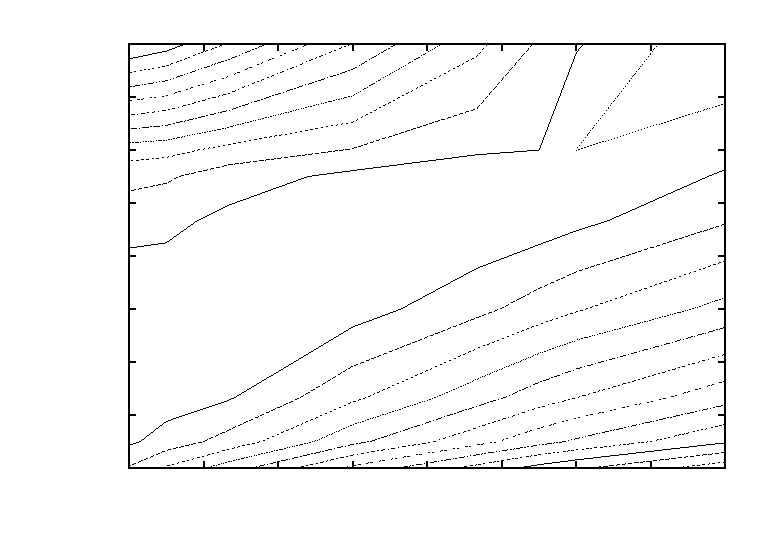
\includegraphics{chapters/chapter6/desertantplot}}%
    \gplfronttext
  \end{picture}%
\endgroup
}
\caption{Contour plot of values for $\sigma$ over values for $r$ and $\tau$ for desert ant foraging}
\label{desertantplot}
\end{figure}


%\begin{figure}
%\input{naiveplot.tex}
%\caption{Contour plot of values for $\sigma$ over values for $r$ and $\tau$ for nai%\"ve foraging}
%\end{figure}

 %But why? Give reason 
%The nai\"ve foraging algorithm slowly clear an entire area around the sink. If there is an equal ratio of robot types to item types then this area would be cleared effectively. 
 %fact that in the more organized environments such as gaussian or vein, it is 

\subsection{Adaptability of the Honey Bee Foraging Algorithm to Item Type Ratio and Comparison to the Na\"ive the Desert Ant Algorithms for Na\"ive and Desert Ant Algorithms}
\label{Adaptability}
Analysis of Table \ref{ratio} indicates that the honey bee foraging algorithm has similar performance throughout all configurations for $r$ and $\tau$, which highlights that the performance of the honey bee algorithm is independent of the configuration of $\tau$, resulting in an algorithm that is more flexible and robust. This could mean that the honey bee algorithm could perform well in dynamic environments where robots and items can be destroyed.

However, according to Table \ref{ratio}, the desert ant algorithm performs better than the honey bee algorithm, for particular configurations of $r$ and $\tau$. This indicates that, if the value of $r$ is known for a particular environment, then it is beneficial to use desert ant foraging and choose $\tau$ appropriately. A possible reason why the desert ant algorithm performs better when optimally configured for a particular environment than the honey bee algorithm is that the honey bee algorithm takes time to adapt to the environment, while the desert ant algorithm with optimal configurations has no division of labour overhead and may outperform the honey bee algorithm under those circumstances.

\section{Scalability}
\label{results:scability}
%Intro

\subsection{Number of Robots}
\label{results:numberenvironments}

%Mann Whitney U tables

%Graphs comparing performance of # of robots, per algorithm,  2 performance measures.
\begin{figure}[!htb]
\centering
\resizebox{\textwidth}{!}{% GNUPLOT: LaTeX picture with Postscript
\begingroup
  \makeatletter
  \providecommand\color[2][]{%
    \GenericError{(gnuplot) \space\space\space\@spaces}{%
      Package color not loaded in conjunction with
      terminal option `colourtext'%
    }{See the gnuplot documentation for explanation.%
    }{Either use 'blacktext' in gnuplot or load the package
      color.sty in LaTeX.}%
    \renewcommand\color[2][]{}%
  }%
  \providecommand\includegraphics[2][]{%
    \GenericError{(gnuplot) \space\space\space\@spaces}{%
      Package graphicx or graphics not loaded%
    }{See the gnuplot documentation for explanation.%
    }{The gnuplot epslatex terminal needs graphicx.sty or graphics.sty.}%
    \renewcommand\includegraphics[2][]{}%
  }%
  \providecommand\rotatebox[2]{#2}%
  \@ifundefined{ifGPcolor}{%
    \newif\ifGPcolor
    \GPcolorfalse
  }{}%
  \@ifundefined{ifGPblacktext}{%
    \newif\ifGPblacktext
    \GPblacktexttrue
  }{}%
  % define a \g@addto@macro without @ in the name:
  \let\gplgaddtomacro\g@addto@macro
  % define empty templates for all commands taking text:
  \gdef\gplbacktext{}%
  \gdef\gplfronttext{}%
  \makeatother
  \ifGPblacktext
    % no textcolor at all
    \def\colorrgb#1{}%
    \def\colorgray#1{}%
  \else
    % gray or color?
    \ifGPcolor
      \def\colorrgb#1{\color[rgb]{#1}}%
      \def\colorgray#1{\color[gray]{#1}}%
      \expandafter\def\csname LTw\endcsname{\color{white}}%
      \expandafter\def\csname LTb\endcsname{\color{black}}%
      \expandafter\def\csname LTa\endcsname{\color{black}}%
      \expandafter\def\csname LT0\endcsname{\color[rgb]{1,0,0}}%
      \expandafter\def\csname LT1\endcsname{\color[rgb]{0,1,0}}%
      \expandafter\def\csname LT2\endcsname{\color[rgb]{0,0,1}}%
      \expandafter\def\csname LT3\endcsname{\color[rgb]{1,0,1}}%
      \expandafter\def\csname LT4\endcsname{\color[rgb]{0,1,1}}%
      \expandafter\def\csname LT5\endcsname{\color[rgb]{1,1,0}}%
      \expandafter\def\csname LT6\endcsname{\color[rgb]{0,0,0}}%
      \expandafter\def\csname LT7\endcsname{\color[rgb]{1,0.3,0}}%
      \expandafter\def\csname LT8\endcsname{\color[rgb]{0.5,0.5,0.5}}%
    \else
      % gray
      \def\colorrgb#1{\color{black}}%
      \def\colorgray#1{\color[gray]{#1}}%
      \expandafter\def\csname LTw\endcsname{\color{white}}%
      \expandafter\def\csname LTb\endcsname{\color{black}}%
      \expandafter\def\csname LTa\endcsname{\color{black}}%
      \expandafter\def\csname LT0\endcsname{\color{black}}%
      \expandafter\def\csname LT1\endcsname{\color{black}}%
      \expandafter\def\csname LT2\endcsname{\color{black}}%
      \expandafter\def\csname LT3\endcsname{\color{black}}%
      \expandafter\def\csname LT4\endcsname{\color{black}}%
      \expandafter\def\csname LT5\endcsname{\color{black}}%
      \expandafter\def\csname LT6\endcsname{\color{black}}%
      \expandafter\def\csname LT7\endcsname{\color{black}}%
      \expandafter\def\csname LT8\endcsname{\color{black}}%
    \fi
  \fi
  \setlength{\unitlength}{0.0500bp}%
  \begin{picture}(7200.00,5040.00)%
    \gplgaddtomacro\gplbacktext{%
      \csname LTb\endcsname%
      \put(1078,704){\makebox(0,0)[r]{\strut{} 0.25}}%
      \put(1078,1163){\makebox(0,0)[r]{\strut{} 0.3}}%
      \put(1078,1623){\makebox(0,0)[r]{\strut{} 0.35}}%
      \put(1078,2082){\makebox(0,0)[r]{\strut{} 0.4}}%
      \put(1078,2541){\makebox(0,0)[r]{\strut{} 0.45}}%
      \put(1078,3001){\makebox(0,0)[r]{\strut{} 0.5}}%
      \put(1078,3460){\makebox(0,0)[r]{\strut{} 0.55}}%
      \put(1078,3920){\makebox(0,0)[r]{\strut{} 0.6}}%
      \put(1078,4379){\makebox(0,0)[r]{\strut{} 0.65}}%
      \put(1210,484){\makebox(0,0){\strut{} 0.1}}%
      \put(1831,484){\makebox(0,0){\strut{} 0.2}}%
      \put(2453,484){\makebox(0,0){\strut{} 0.3}}%
      \put(3074,484){\makebox(0,0){\strut{} 0.4}}%
      \put(3696,484){\makebox(0,0){\strut{} 0.5}}%
      \put(4317,484){\makebox(0,0){\strut{} 0.6}}%
      \put(4939,484){\makebox(0,0){\strut{} 0.7}}%
      \put(5560,484){\makebox(0,0){\strut{} 0.8}}%
      \put(6182,484){\makebox(0,0){\strut{} 0.9}}%
      \put(6803,484){\makebox(0,0){\strut{} 1.0}}%
      \put(176,2541){\rotatebox{-270}{\makebox(0,0){\strut{}Prioritized items over time ($\sigma$)}}}%
      \put(4006,154){\makebox(0,0){\strut{}Swarm Density($c$)}}%
      \put(4006,4709){\makebox(0,0){\strut{}Prioritized items over time for each algorithm over swarm density}}%
    }%
    \gplgaddtomacro\gplfronttext{%
      \csname LTb\endcsname%
      \put(5816,4206){\makebox(0,0)[r]{\strut{}Na\"ive}}%
      \csname LTb\endcsname%
      \put(5816,3986){\makebox(0,0)[r]{\strut{}Desert Ant}}%
      \csname LTb\endcsname%
      \put(5816,3766){\makebox(0,0)[r]{\strut{}Honey Bee}}%
    }%
    \gplbacktext
    \put(0,0){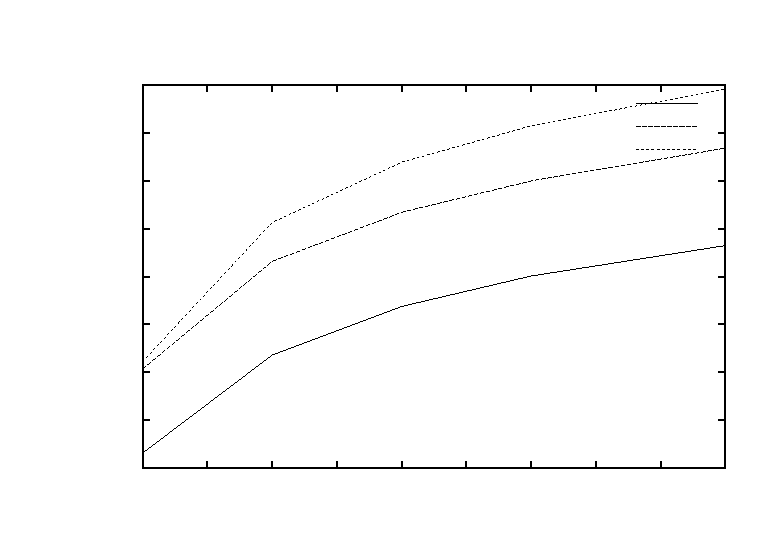
\includegraphics{chapters/chapter6/graphs/gold_robots}}%
    \gplfronttext
  \end{picture}%
\endgroup
}
\caption{Number of Robots }
\label{robotsgoldplot}
\end{figure}

\begin{figure}[!htb]
\centering
\resizebox{\textwidth}{!}{% GNUPLOT: LaTeX picture with Postscript
\begingroup
  \makeatletter
  \providecommand\color[2][]{%
    \GenericError{(gnuplot) \space\space\space\@spaces}{%
      Package color not loaded in conjunction with
      terminal option `colourtext'%
    }{See the gnuplot documentation for explanation.%
    }{Either use 'blacktext' in gnuplot or load the package
      color.sty in LaTeX.}%
    \renewcommand\color[2][]{}%
  }%
  \providecommand\includegraphics[2][]{%
    \GenericError{(gnuplot) \space\space\space\@spaces}{%
      Package graphicx or graphics not loaded%
    }{See the gnuplot documentation for explanation.%
    }{The gnuplot epslatex terminal needs graphicx.sty or graphics.sty.}%
    \renewcommand\includegraphics[2][]{}%
  }%
  \providecommand\rotatebox[2]{#2}%
  \@ifundefined{ifGPcolor}{%
    \newif\ifGPcolor
    \GPcolorfalse
  }{}%
  \@ifundefined{ifGPblacktext}{%
    \newif\ifGPblacktext
    \GPblacktexttrue
  }{}%
  % define a \g@addto@macro without @ in the name:
  \let\gplgaddtomacro\g@addto@macro
  % define empty templates for all commands taking text:
  \gdef\gplbacktext{}%
  \gdef\gplfronttext{}%
  \makeatother
  \ifGPblacktext
    % no textcolor at all
    \def\colorrgb#1{}%
    \def\colorgray#1{}%
  \else
    % gray or color?
    \ifGPcolor
      \def\colorrgb#1{\color[rgb]{#1}}%
      \def\colorgray#1{\color[gray]{#1}}%
      \expandafter\def\csname LTw\endcsname{\color{white}}%
      \expandafter\def\csname LTb\endcsname{\color{black}}%
      \expandafter\def\csname LTa\endcsname{\color{black}}%
      \expandafter\def\csname LT0\endcsname{\color[rgb]{1,0,0}}%
      \expandafter\def\csname LT1\endcsname{\color[rgb]{0,1,0}}%
      \expandafter\def\csname LT2\endcsname{\color[rgb]{0,0,1}}%
      \expandafter\def\csname LT3\endcsname{\color[rgb]{1,0,1}}%
      \expandafter\def\csname LT4\endcsname{\color[rgb]{0,1,1}}%
      \expandafter\def\csname LT5\endcsname{\color[rgb]{1,1,0}}%
      \expandafter\def\csname LT6\endcsname{\color[rgb]{0,0,0}}%
      \expandafter\def\csname LT7\endcsname{\color[rgb]{1,0.3,0}}%
      \expandafter\def\csname LT8\endcsname{\color[rgb]{0.5,0.5,0.5}}%
    \else
      % gray
      \def\colorrgb#1{\color{black}}%
      \def\colorgray#1{\color[gray]{#1}}%
      \expandafter\def\csname LTw\endcsname{\color{white}}%
      \expandafter\def\csname LTb\endcsname{\color{black}}%
      \expandafter\def\csname LTa\endcsname{\color{black}}%
      \expandafter\def\csname LT0\endcsname{\color{black}}%
      \expandafter\def\csname LT1\endcsname{\color{black}}%
      \expandafter\def\csname LT2\endcsname{\color{black}}%
      \expandafter\def\csname LT3\endcsname{\color{black}}%
      \expandafter\def\csname LT4\endcsname{\color{black}}%
      \expandafter\def\csname LT5\endcsname{\color{black}}%
      \expandafter\def\csname LT6\endcsname{\color{black}}%
      \expandafter\def\csname LT7\endcsname{\color{black}}%
      \expandafter\def\csname LT8\endcsname{\color{black}}%
    \fi
  \fi
  \setlength{\unitlength}{0.0500bp}%
  \begin{picture}(7200.00,5040.00)%
    \gplgaddtomacro\gplbacktext{%
      \csname LTb\endcsname%
      \put(1078,704){\makebox(0,0)[r]{\strut{} 0.25}}%
      \put(1078,1071){\makebox(0,0)[r]{\strut{} 0.3}}%
      \put(1078,1439){\makebox(0,0)[r]{\strut{} 0.35}}%
      \put(1078,1806){\makebox(0,0)[r]{\strut{} 0.4}}%
      \put(1078,2174){\makebox(0,0)[r]{\strut{} 0.45}}%
      \put(1078,2541){\makebox(0,0)[r]{\strut{} 0.5}}%
      \put(1078,2909){\makebox(0,0)[r]{\strut{} 0.55}}%
      \put(1078,3276){\makebox(0,0)[r]{\strut{} 0.6}}%
      \put(1078,3644){\makebox(0,0)[r]{\strut{} 0.65}}%
      \put(1078,4012){\makebox(0,0)[r]{\strut{} 0.7}}%
      \put(1078,4379){\makebox(0,0)[r]{\strut{} 0.75}}%
      \put(1210,484){\makebox(0,0){\strut{} 0}}%
      \put(1831,484){\makebox(0,0){\strut{} 10}}%
      \put(2453,484){\makebox(0,0){\strut{} 20}}%
      \put(3074,484){\makebox(0,0){\strut{} 30}}%
      \put(3696,484){\makebox(0,0){\strut{} 40}}%
      \put(4317,484){\makebox(0,0){\strut{} 50}}%
      \put(4939,484){\makebox(0,0){\strut{} 60}}%
      \put(5560,484){\makebox(0,0){\strut{} 70}}%
      \put(6182,484){\makebox(0,0){\strut{} 80}}%
      \put(6803,484){\makebox(0,0){\strut{} 90}}%
      \put(176,2541){\rotatebox{-270}{\makebox(0,0){\strut{}Non-prioritized items over time ($\sigma$)}}}%
      \put(4006,154){\makebox(0,0){\strut{}Quantity of Robots ($c$)}}%
      \put(4006,4709){\makebox(0,0){\strut{}Non-prioritized items over time for each algorithm over robot percentages}}%
    }%
    \gplgaddtomacro\gplfronttext{%
      \csname LTb\endcsname%
      \put(5816,4206){\makebox(0,0)[r]{\strut{}Na\"ive}}%
      \csname LTb\endcsname%
      \put(5816,3986){\makebox(0,0)[r]{\strut{}Desert Ant}}%
      \csname LTb\endcsname%
      \put(5816,3766){\makebox(0,0)[r]{\strut{}Honey Bee}}%
    }%
    \gplbacktext
    \put(0,0){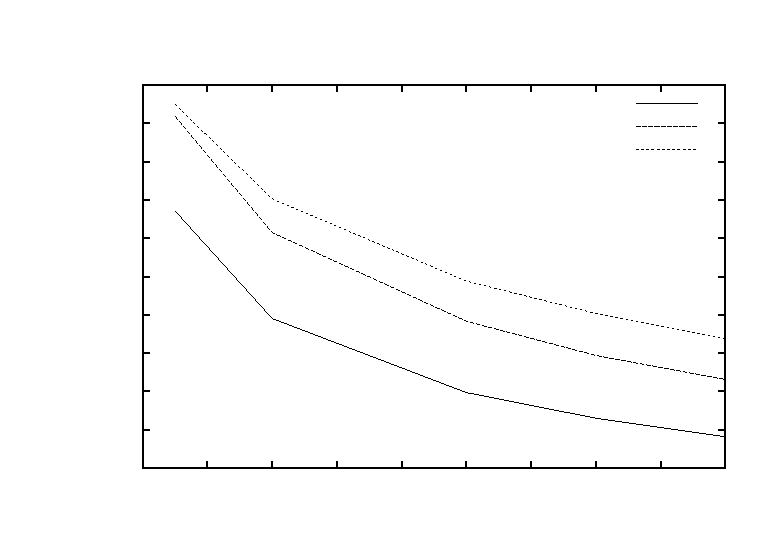
\includegraphics{chapters/chapter6/graphs/waste_robots}}%
    \gplfronttext
  \end{picture}%
\endgroup
}
\caption{Non-prioritized items over time over number of Robots}
\label{robotswasteplot}
\end{figure}

%Discussion
The purpose of examining the effect of additional robots is to determine whether the addition of extra robots negatively effects the algorithm's performance. An algorithm that would scale perfectly would show a linear increase in performance as the number of robots increases. A slow down in the rate of improvement could mean a few things 
\begin{enumerate}
\item That the robots manage to successfully forage the entire environment and thus addition of robots makes no difference.
\item That the addition of more robots creates interference between the robots or causes malfunction within the algorithms thus impacting scalability. 
\end{enumerate}


The graph displays the  logorithmic trendline, the equation of the trendline and the value of the coefficient of determination,$r^2$, is shown. The graph shows that the performance of the algorithms increase logarithmically as more robots are added with a $p$-value of 0.05. 

Honey-bee has the greatest slope which means it is least negatively affected by the increase in robots, followed by desert ant soon after and na\"ive foraging being the most effected by an increase in robots


\subsection{Energy}
\label{results:energy}

%Graph for energy saved by honey bee algorithm. Similar performance. 

%Due to the waiting state, the honey bee algorithm should  saving energy and thus be more energy efficient. The amount of time spent in a waiting state was measured, however surprisingly, not much time was spent waiting overall. This indicates that there is room for improvement from an energy perspective.

\subsection{Environment Size}
\label{results:environmentsize}

%As environment size increases, how does the algorithm performance suffer

%Mann whitney U + average etc etc
%Graphs compareing performacne of # robots, per algorith, for each performance measure 2 performance measures

\begin{figure}[!htb]
\centering
\resizebox{\textwidth}{!}{% GNUPLOT: LaTeX picture with Postscript
\begingroup
  \makeatletter
  \providecommand\color[2][]{%
    \GenericError{(gnuplot) \space\space\space\@spaces}{%
      Package color not loaded in conjunction with
      terminal option `colourtext'%
    }{See the gnuplot documentation for explanation.%
    }{Either use 'blacktext' in gnuplot or load the package
      color.sty in LaTeX.}%
    \renewcommand\color[2][]{}%
  }%
  \providecommand\includegraphics[2][]{%
    \GenericError{(gnuplot) \space\space\space\@spaces}{%
      Package graphicx or graphics not loaded%
    }{See the gnuplot documentation for explanation.%
    }{The gnuplot epslatex terminal needs graphicx.sty or graphics.sty.}%
    \renewcommand\includegraphics[2][]{}%
  }%
  \providecommand\rotatebox[2]{#2}%
  \@ifundefined{ifGPcolor}{%
    \newif\ifGPcolor
    \GPcolorfalse
  }{}%
  \@ifundefined{ifGPblacktext}{%
    \newif\ifGPblacktext
    \GPblacktexttrue
  }{}%
  % define a \g@addto@macro without @ in the name:
  \let\gplgaddtomacro\g@addto@macro
  % define empty templates for all commands taking text:
  \gdef\gplbacktext{}%
  \gdef\gplfronttext{}%
  \makeatother
  \ifGPblacktext
    % no textcolor at all
    \def\colorrgb#1{}%
    \def\colorgray#1{}%
  \else
    % gray or color?
    \ifGPcolor
      \def\colorrgb#1{\color[rgb]{#1}}%
      \def\colorgray#1{\color[gray]{#1}}%
      \expandafter\def\csname LTw\endcsname{\color{white}}%
      \expandafter\def\csname LTb\endcsname{\color{black}}%
      \expandafter\def\csname LTa\endcsname{\color{black}}%
      \expandafter\def\csname LT0\endcsname{\color[rgb]{1,0,0}}%
      \expandafter\def\csname LT1\endcsname{\color[rgb]{0,1,0}}%
      \expandafter\def\csname LT2\endcsname{\color[rgb]{0,0,1}}%
      \expandafter\def\csname LT3\endcsname{\color[rgb]{1,0,1}}%
      \expandafter\def\csname LT4\endcsname{\color[rgb]{0,1,1}}%
      \expandafter\def\csname LT5\endcsname{\color[rgb]{1,1,0}}%
      \expandafter\def\csname LT6\endcsname{\color[rgb]{0,0,0}}%
      \expandafter\def\csname LT7\endcsname{\color[rgb]{1,0.3,0}}%
      \expandafter\def\csname LT8\endcsname{\color[rgb]{0.5,0.5,0.5}}%
    \else
      % gray
      \def\colorrgb#1{\color{black}}%
      \def\colorgray#1{\color[gray]{#1}}%
      \expandafter\def\csname LTw\endcsname{\color{white}}%
      \expandafter\def\csname LTb\endcsname{\color{black}}%
      \expandafter\def\csname LTa\endcsname{\color{black}}%
      \expandafter\def\csname LT0\endcsname{\color{black}}%
      \expandafter\def\csname LT1\endcsname{\color{black}}%
      \expandafter\def\csname LT2\endcsname{\color{black}}%
      \expandafter\def\csname LT3\endcsname{\color{black}}%
      \expandafter\def\csname LT4\endcsname{\color{black}}%
      \expandafter\def\csname LT5\endcsname{\color{black}}%
      \expandafter\def\csname LT6\endcsname{\color{black}}%
      \expandafter\def\csname LT7\endcsname{\color{black}}%
      \expandafter\def\csname LT8\endcsname{\color{black}}%
    \fi
  \fi
  \setlength{\unitlength}{0.0500bp}%
  \begin{picture}(7200.00,5040.00)%
    \gplgaddtomacro\gplbacktext{%
      \csname LTb\endcsname%
      \put(946,704){\makebox(0,0)[r]{\strut{} 0.1}}%
      \put(946,1112){\makebox(0,0)[r]{\strut{} 0.2}}%
      \put(946,1521){\makebox(0,0)[r]{\strut{} 0.3}}%
      \put(946,1929){\makebox(0,0)[r]{\strut{} 0.4}}%
      \put(946,2337){\makebox(0,0)[r]{\strut{} 0.5}}%
      \put(946,2746){\makebox(0,0)[r]{\strut{} 0.6}}%
      \put(946,3154){\makebox(0,0)[r]{\strut{} 0.7}}%
      \put(946,3562){\makebox(0,0)[r]{\strut{} 0.8}}%
      \put(946,3971){\makebox(0,0)[r]{\strut{} 0.9}}%
      \put(946,4379){\makebox(0,0)[r]{\strut{} 1}}%
      \put(1078,484){\makebox(0,0){\strut{} 50}}%
      \put(1714,484){\makebox(0,0){\strut{} 100}}%
      \put(2350,484){\makebox(0,0){\strut{} 150}}%
      \put(2986,484){\makebox(0,0){\strut{} 200}}%
      \put(3622,484){\makebox(0,0){\strut{} 250}}%
      \put(4259,484){\makebox(0,0){\strut{} 300}}%
      \put(4895,484){\makebox(0,0){\strut{} 350}}%
      \put(5531,484){\makebox(0,0){\strut{} 400}}%
      \put(6167,484){\makebox(0,0){\strut{} 450}}%
      \put(6803,484){\makebox(0,0){\strut{} 500}}%
      \put(176,2541){\rotatebox{-270}{\makebox(0,0){\strut{}Prioritized items over time ($\sigma$)}}}%
      \put(3940,154){\makebox(0,0){\strut{}Size ($S$)}}%
      \put(3940,4709){\makebox(0,0){\strut{}Prioritized items over time for each algorithm for different grid sizes}}%
    }%
    \gplgaddtomacro\gplfronttext{%
      \csname LTb\endcsname%
      \put(5816,4206){\makebox(0,0)[r]{\strut{}Na\"ive}}%
      \csname LTb\endcsname%
      \put(5816,3986){\makebox(0,0)[r]{\strut{}Desert Ant}}%
      \csname LTb\endcsname%
      \put(5816,3766){\makebox(0,0)[r]{\strut{}Honey Bee}}%
    }%
    \gplbacktext
    \put(0,0){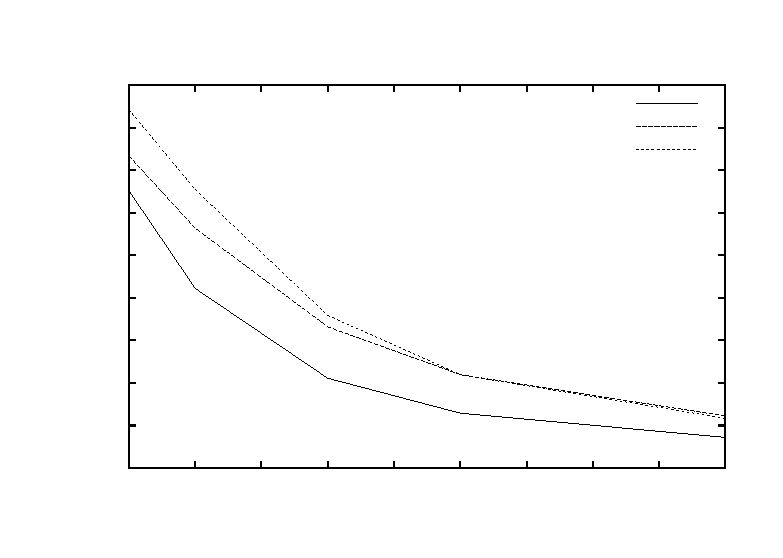
\includegraphics{chapters/chapter6/graphs/gold_sizes}}%
    \gplfronttext
  \end{picture}%
\endgroup
}
\caption{Sizes of Environment }
\label{sizegoldplot}
\end{figure}

\begin{figure}[!htb]
\centering
\resizebox{\textwidth}{!}{% GNUPLOT: LaTeX picture with Postscript
\begingroup
  \makeatletter
  \providecommand\color[2][]{%
    \GenericError{(gnuplot) \space\space\space\@spaces}{%
      Package color not loaded in conjunction with
      terminal option `colourtext'%
    }{See the gnuplot documentation for explanation.%
    }{Either use 'blacktext' in gnuplot or load the package
      color.sty in LaTeX.}%
    \renewcommand\color[2][]{}%
  }%
  \providecommand\includegraphics[2][]{%
    \GenericError{(gnuplot) \space\space\space\@spaces}{%
      Package graphicx or graphics not loaded%
    }{See the gnuplot documentation for explanation.%
    }{The gnuplot epslatex terminal needs graphicx.sty or graphics.sty.}%
    \renewcommand\includegraphics[2][]{}%
  }%
  \providecommand\rotatebox[2]{#2}%
  \@ifundefined{ifGPcolor}{%
    \newif\ifGPcolor
    \GPcolorfalse
  }{}%
  \@ifundefined{ifGPblacktext}{%
    \newif\ifGPblacktext
    \GPblacktexttrue
  }{}%
  % define a \g@addto@macro without @ in the name:
  \let\gplgaddtomacro\g@addto@macro
  % define empty templates for all commands taking text:
  \gdef\gplbacktext{}%
  \gdef\gplfronttext{}%
  \makeatother
  \ifGPblacktext
    % no textcolor at all
    \def\colorrgb#1{}%
    \def\colorgray#1{}%
  \else
    % gray or color?
    \ifGPcolor
      \def\colorrgb#1{\color[rgb]{#1}}%
      \def\colorgray#1{\color[gray]{#1}}%
      \expandafter\def\csname LTw\endcsname{\color{white}}%
      \expandafter\def\csname LTb\endcsname{\color{black}}%
      \expandafter\def\csname LTa\endcsname{\color{black}}%
      \expandafter\def\csname LT0\endcsname{\color[rgb]{1,0,0}}%
      \expandafter\def\csname LT1\endcsname{\color[rgb]{0,1,0}}%
      \expandafter\def\csname LT2\endcsname{\color[rgb]{0,0,1}}%
      \expandafter\def\csname LT3\endcsname{\color[rgb]{1,0,1}}%
      \expandafter\def\csname LT4\endcsname{\color[rgb]{0,1,1}}%
      \expandafter\def\csname LT5\endcsname{\color[rgb]{1,1,0}}%
      \expandafter\def\csname LT6\endcsname{\color[rgb]{0,0,0}}%
      \expandafter\def\csname LT7\endcsname{\color[rgb]{1,0.3,0}}%
      \expandafter\def\csname LT8\endcsname{\color[rgb]{0.5,0.5,0.5}}%
    \else
      % gray
      \def\colorrgb#1{\color{black}}%
      \def\colorgray#1{\color[gray]{#1}}%
      \expandafter\def\csname LTw\endcsname{\color{white}}%
      \expandafter\def\csname LTb\endcsname{\color{black}}%
      \expandafter\def\csname LTa\endcsname{\color{black}}%
      \expandafter\def\csname LT0\endcsname{\color{black}}%
      \expandafter\def\csname LT1\endcsname{\color{black}}%
      \expandafter\def\csname LT2\endcsname{\color{black}}%
      \expandafter\def\csname LT3\endcsname{\color{black}}%
      \expandafter\def\csname LT4\endcsname{\color{black}}%
      \expandafter\def\csname LT5\endcsname{\color{black}}%
      \expandafter\def\csname LT6\endcsname{\color{black}}%
      \expandafter\def\csname LT7\endcsname{\color{black}}%
      \expandafter\def\csname LT8\endcsname{\color{black}}%
    \fi
  \fi
  \setlength{\unitlength}{0.0500bp}%
  \begin{picture}(7200.00,5040.00)%
    \gplgaddtomacro\gplbacktext{%
      \csname LTb\endcsname%
      \put(946,704){\makebox(0,0)[r]{\strut{} 0.1}}%
      \put(946,1112){\makebox(0,0)[r]{\strut{} 0.2}}%
      \put(946,1521){\makebox(0,0)[r]{\strut{} 0.3}}%
      \put(946,1929){\makebox(0,0)[r]{\strut{} 0.4}}%
      \put(946,2337){\makebox(0,0)[r]{\strut{} 0.5}}%
      \put(946,2746){\makebox(0,0)[r]{\strut{} 0.6}}%
      \put(946,3154){\makebox(0,0)[r]{\strut{} 0.7}}%
      \put(946,3562){\makebox(0,0)[r]{\strut{} 0.8}}%
      \put(946,3971){\makebox(0,0)[r]{\strut{} 0.9}}%
      \put(946,4379){\makebox(0,0)[r]{\strut{} 1}}%
      \put(1078,484){\makebox(0,0){\strut{} 50}}%
      \put(1714,484){\makebox(0,0){\strut{} 100}}%
      \put(2350,484){\makebox(0,0){\strut{} 150}}%
      \put(2986,484){\makebox(0,0){\strut{} 200}}%
      \put(3622,484){\makebox(0,0){\strut{} 250}}%
      \put(4259,484){\makebox(0,0){\strut{} 300}}%
      \put(4895,484){\makebox(0,0){\strut{} 350}}%
      \put(5531,484){\makebox(0,0){\strut{} 400}}%
      \put(6167,484){\makebox(0,0){\strut{} 450}}%
      \put(6803,484){\makebox(0,0){\strut{} 500}}%
      \put(176,2541){\rotatebox{-270}{\makebox(0,0){\strut{}Non-prioritized items over time ($\sigma$)}}}%
      \put(3940,154){\makebox(0,0){\strut{}Size ($S$)}}%
      \put(3940,4709){\makebox(0,0){\strut{}Non-prioritized items over time for each algorithm for different grid sizes}}%
    }%
    \gplgaddtomacro\gplfronttext{%
      \csname LTb\endcsname%
      \put(5816,4206){\makebox(0,0)[r]{\strut{}Na\"ive}}%
      \csname LTb\endcsname%
      \put(5816,3986){\makebox(0,0)[r]{\strut{}Desert Ant}}%
      \csname LTb\endcsname%
      \put(5816,3766){\makebox(0,0)[r]{\strut{}Honey Bee}}%
    }%
    \gplbacktext
    \put(0,0){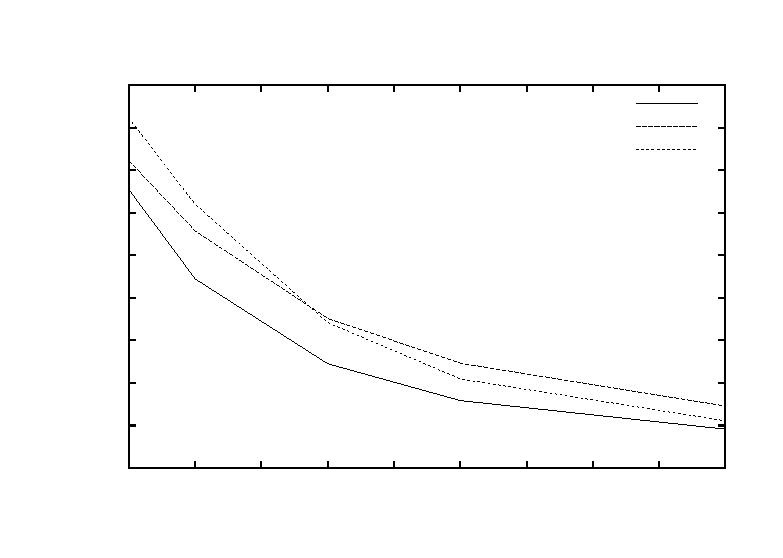
\includegraphics{chapters/chapter6/graphs/waste_sizes}}%
    \gplfronttext
  \end{picture}%
\endgroup
}
\caption{Non-prioritized items over time over sizes of Environment for each algorithm}
\label{sizewasteplot}
\end{figure}
%Discussion
It should be noted that as the robot size increases, that the number of robots assigned to each environment will also increase since the number of robots is based on a percentage of $S$, the environment size.
As the environment size increases, one would expect the performance to get quadratically smaller since the algorithms were run for the same amount of time. I'm not sure how this can be attributed to scalability. 

\section{Flexibility}
\label{results:flexibility}

%Intro description

\subsection{Ratio}
\label{results:ratio}
%How is are the algorithms affected by changes in ratio. 

%Mann-WHitney U & average
%Graphs comparing performance of ratio

\begin{figure}[!htb]
\centering
\resizebox{\textwidth}{!}{% GNUPLOT: LaTeX picture with Postscript
\begingroup
  \makeatletter
  \providecommand\color[2][]{%
    \GenericError{(gnuplot) \space\space\space\@spaces}{%
      Package color not loaded in conjunction with
      terminal option `colourtext'%
    }{See the gnuplot documentation for explanation.%
    }{Either use 'blacktext' in gnuplot or load the package
      color.sty in LaTeX.}%
    \renewcommand\color[2][]{}%
  }%
  \providecommand\includegraphics[2][]{%
    \GenericError{(gnuplot) \space\space\space\@spaces}{%
      Package graphicx or graphics not loaded%
    }{See the gnuplot documentation for explanation.%
    }{The gnuplot epslatex terminal needs graphicx.sty or graphics.sty.}%
    \renewcommand\includegraphics[2][]{}%
  }%
  \providecommand\rotatebox[2]{#2}%
  \@ifundefined{ifGPcolor}{%
    \newif\ifGPcolor
    \GPcolorfalse
  }{}%
  \@ifundefined{ifGPblacktext}{%
    \newif\ifGPblacktext
    \GPblacktexttrue
  }{}%
  % define a \g@addto@macro without @ in the name:
  \let\gplgaddtomacro\g@addto@macro
  % define empty templates for all commands taking text:
  \gdef\gplbacktext{}%
  \gdef\gplfronttext{}%
  \makeatother
  \ifGPblacktext
    % no textcolor at all
    \def\colorrgb#1{}%
    \def\colorgray#1{}%
  \else
    % gray or color?
    \ifGPcolor
      \def\colorrgb#1{\color[rgb]{#1}}%
      \def\colorgray#1{\color[gray]{#1}}%
      \expandafter\def\csname LTw\endcsname{\color{white}}%
      \expandafter\def\csname LTb\endcsname{\color{black}}%
      \expandafter\def\csname LTa\endcsname{\color{black}}%
      \expandafter\def\csname LT0\endcsname{\color[rgb]{1,0,0}}%
      \expandafter\def\csname LT1\endcsname{\color[rgb]{0,1,0}}%
      \expandafter\def\csname LT2\endcsname{\color[rgb]{0,0,1}}%
      \expandafter\def\csname LT3\endcsname{\color[rgb]{1,0,1}}%
      \expandafter\def\csname LT4\endcsname{\color[rgb]{0,1,1}}%
      \expandafter\def\csname LT5\endcsname{\color[rgb]{1,1,0}}%
      \expandafter\def\csname LT6\endcsname{\color[rgb]{0,0,0}}%
      \expandafter\def\csname LT7\endcsname{\color[rgb]{1,0.3,0}}%
      \expandafter\def\csname LT8\endcsname{\color[rgb]{0.5,0.5,0.5}}%
    \else
      % gray
      \def\colorrgb#1{\color{black}}%
      \def\colorgray#1{\color[gray]{#1}}%
      \expandafter\def\csname LTw\endcsname{\color{white}}%
      \expandafter\def\csname LTb\endcsname{\color{black}}%
      \expandafter\def\csname LTa\endcsname{\color{black}}%
      \expandafter\def\csname LT0\endcsname{\color{black}}%
      \expandafter\def\csname LT1\endcsname{\color{black}}%
      \expandafter\def\csname LT2\endcsname{\color{black}}%
      \expandafter\def\csname LT3\endcsname{\color{black}}%
      \expandafter\def\csname LT4\endcsname{\color{black}}%
      \expandafter\def\csname LT5\endcsname{\color{black}}%
      \expandafter\def\csname LT6\endcsname{\color{black}}%
      \expandafter\def\csname LT7\endcsname{\color{black}}%
      \expandafter\def\csname LT8\endcsname{\color{black}}%
    \fi
  \fi
  \setlength{\unitlength}{0.0500bp}%
  \begin{picture}(7200.00,5040.00)%
    \gplgaddtomacro\gplbacktext{%
      \csname LTb\endcsname%
      \put(946,704){\makebox(0,0)[r]{\strut{} 0.3}}%
      \put(946,1229){\makebox(0,0)[r]{\strut{} 0.4}}%
      \put(946,1754){\makebox(0,0)[r]{\strut{} 0.5}}%
      \put(946,2279){\makebox(0,0)[r]{\strut{} 0.6}}%
      \put(946,2804){\makebox(0,0)[r]{\strut{} 0.7}}%
      \put(946,3329){\makebox(0,0)[r]{\strut{} 0.8}}%
      \put(946,3854){\makebox(0,0)[r]{\strut{} 0.9}}%
      \put(946,4379){\makebox(0,0)[r]{\strut{} 1}}%
      \put(1078,484){\makebox(0,0){\strut{} 0}}%
      \put(2223,484){\makebox(0,0){\strut{} 0.2}}%
      \put(3368,484){\makebox(0,0){\strut{} 0.4}}%
      \put(4513,484){\makebox(0,0){\strut{} 0.6}}%
      \put(5658,484){\makebox(0,0){\strut{} 0.8}}%
      \put(6803,484){\makebox(0,0){\strut{} 1}}%
      \put(176,2541){\rotatebox{-270}{\makebox(0,0){\strut{}Prioritized items over time ($\sigma$)}}}%
      \put(3940,154){\makebox(0,0){\strut{}Item Type Ratio ($r$)}}%
      \put(3940,4709){\makebox(0,0){\strut{}Prioritized items over time for each algorithm for item type ratios}}%
    }%
    \gplgaddtomacro\gplfronttext{%
      \csname LTb\endcsname%
      \put(5816,4206){\makebox(0,0)[r]{\strut{}Na\"ive}}%
      \csname LTb\endcsname%
      \put(5816,3986){\makebox(0,0)[r]{\strut{}Desert Ant}}%
      \csname LTb\endcsname%
      \put(5816,3766){\makebox(0,0)[r]{\strut{}Honey Bee}}%
    }%
    \gplbacktext
    \put(0,0){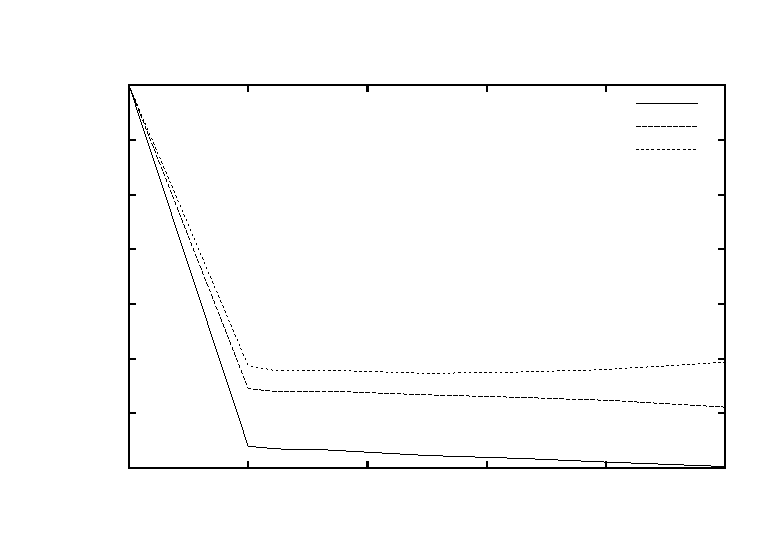
\includegraphics{chapters/chapter6/graphs/gold_ratio}}%
    \gplfronttext
  \end{picture}%
\endgroup
}
\caption{Prioritized items over time over ratio of Items in Environment for each algorithm }
\label{ratiogoldplot}
\end{figure}


\begin{figure}[!htb]
\centering
\resizebox{\textwidth}{!}{% GNUPLOT: LaTeX picture with Postscript
\begingroup
  \makeatletter
  \providecommand\color[2][]{%
    \GenericError{(gnuplot) \space\space\space\@spaces}{%
      Package color not loaded in conjunction with
      terminal option `colourtext'%
    }{See the gnuplot documentation for explanation.%
    }{Either use 'blacktext' in gnuplot or load the package
      color.sty in LaTeX.}%
    \renewcommand\color[2][]{}%
  }%
  \providecommand\includegraphics[2][]{%
    \GenericError{(gnuplot) \space\space\space\@spaces}{%
      Package graphicx or graphics not loaded%
    }{See the gnuplot documentation for explanation.%
    }{The gnuplot epslatex terminal needs graphicx.sty or graphics.sty.}%
    \renewcommand\includegraphics[2][]{}%
  }%
  \providecommand\rotatebox[2]{#2}%
  \@ifundefined{ifGPcolor}{%
    \newif\ifGPcolor
    \GPcolorfalse
  }{}%
  \@ifundefined{ifGPblacktext}{%
    \newif\ifGPblacktext
    \GPblacktexttrue
  }{}%
  % define a \g@addto@macro without @ in the name:
  \let\gplgaddtomacro\g@addto@macro
  % define empty templates for all commands taking text:
  \gdef\gplbacktext{}%
  \gdef\gplfronttext{}%
  \makeatother
  \ifGPblacktext
    % no textcolor at all
    \def\colorrgb#1{}%
    \def\colorgray#1{}%
  \else
    % gray or color?
    \ifGPcolor
      \def\colorrgb#1{\color[rgb]{#1}}%
      \def\colorgray#1{\color[gray]{#1}}%
      \expandafter\def\csname LTw\endcsname{\color{white}}%
      \expandafter\def\csname LTb\endcsname{\color{black}}%
      \expandafter\def\csname LTa\endcsname{\color{black}}%
      \expandafter\def\csname LT0\endcsname{\color[rgb]{1,0,0}}%
      \expandafter\def\csname LT1\endcsname{\color[rgb]{0,1,0}}%
      \expandafter\def\csname LT2\endcsname{\color[rgb]{0,0,1}}%
      \expandafter\def\csname LT3\endcsname{\color[rgb]{1,0,1}}%
      \expandafter\def\csname LT4\endcsname{\color[rgb]{0,1,1}}%
      \expandafter\def\csname LT5\endcsname{\color[rgb]{1,1,0}}%
      \expandafter\def\csname LT6\endcsname{\color[rgb]{0,0,0}}%
      \expandafter\def\csname LT7\endcsname{\color[rgb]{1,0.3,0}}%
      \expandafter\def\csname LT8\endcsname{\color[rgb]{0.5,0.5,0.5}}%
    \else
      % gray
      \def\colorrgb#1{\color{black}}%
      \def\colorgray#1{\color[gray]{#1}}%
      \expandafter\def\csname LTw\endcsname{\color{white}}%
      \expandafter\def\csname LTb\endcsname{\color{black}}%
      \expandafter\def\csname LTa\endcsname{\color{black}}%
      \expandafter\def\csname LT0\endcsname{\color{black}}%
      \expandafter\def\csname LT1\endcsname{\color{black}}%
      \expandafter\def\csname LT2\endcsname{\color{black}}%
      \expandafter\def\csname LT3\endcsname{\color{black}}%
      \expandafter\def\csname LT4\endcsname{\color{black}}%
      \expandafter\def\csname LT5\endcsname{\color{black}}%
      \expandafter\def\csname LT6\endcsname{\color{black}}%
      \expandafter\def\csname LT7\endcsname{\color{black}}%
      \expandafter\def\csname LT8\endcsname{\color{black}}%
    \fi
  \fi
  \setlength{\unitlength}{0.0500bp}%
  \begin{picture}(7200.00,5040.00)%
    \gplgaddtomacro\gplbacktext{%
      \csname LTb\endcsname%
      \put(946,704){\makebox(0,0)[r]{\strut{} 0.3}}%
      \put(946,1229){\makebox(0,0)[r]{\strut{} 0.4}}%
      \put(946,1754){\makebox(0,0)[r]{\strut{} 0.5}}%
      \put(946,2279){\makebox(0,0)[r]{\strut{} 0.6}}%
      \put(946,2804){\makebox(0,0)[r]{\strut{} 0.7}}%
      \put(946,3329){\makebox(0,0)[r]{\strut{} 0.8}}%
      \put(946,3854){\makebox(0,0)[r]{\strut{} 0.9}}%
      \put(946,4379){\makebox(0,0)[r]{\strut{} 1}}%
      \put(1078,484){\makebox(0,0){\strut{} 0}}%
      \put(2223,484){\makebox(0,0){\strut{} 0.2}}%
      \put(3368,484){\makebox(0,0){\strut{} 0.4}}%
      \put(4513,484){\makebox(0,0){\strut{} 0.6}}%
      \put(5658,484){\makebox(0,0){\strut{} 0.8}}%
      \put(6803,484){\makebox(0,0){\strut{} 1}}%
      \put(176,2541){\rotatebox{-270}{\makebox(0,0){\strut{}Non-prioritized items over time ($\sigma$)}}}%
      \put(3940,154){\makebox(0,0){\strut{}Item Type Ratio ($r$)}}%
      \put(3940,4709){\makebox(0,0){\strut{}Non-prioritized items over time for each algorithm for item type ratios}}%
    }%
    \gplgaddtomacro\gplfronttext{%
      \csname LTb\endcsname%
      \put(5816,4206){\makebox(0,0)[r]{\strut{}Na\"ive}}%
      \csname LTb\endcsname%
      \put(5816,3986){\makebox(0,0)[r]{\strut{}Desert Ant}}%
      \csname LTb\endcsname%
      \put(5816,3766){\makebox(0,0)[r]{\strut{}Honey Bee}}%
    }%
    \gplbacktext
    \put(0,0){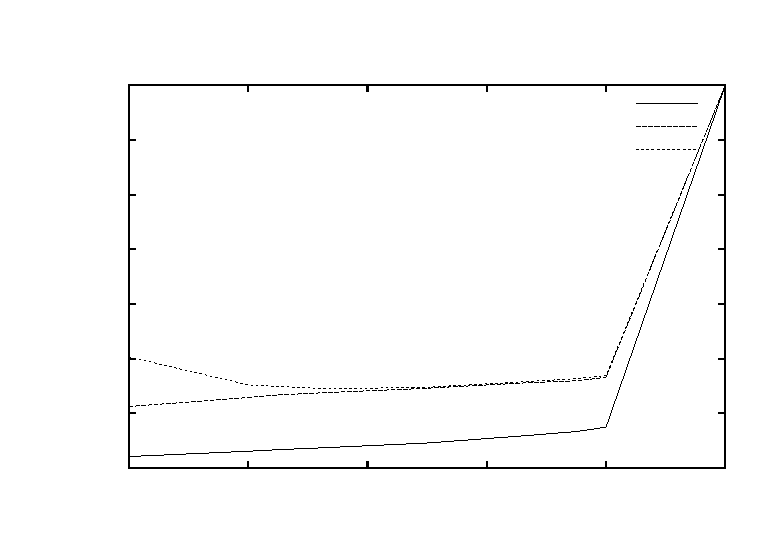
\includegraphics{chapters/chapter6/graphs/waste_ratio}}%
    \gplfronttext
  \end{picture}%
\endgroup
}
\caption{Non-prioritized items over time over ratio of Items in Environment for each algorithm}
\label{ratiowasteplot}
\end{figure}

%Discussion
Ratio has to be analysed within the context of division. Even so - very minimal effect makes me wonder. 
\subsection{Environmental Types}
\label{results:environmentaltypes}

%How are the algorithms affected by changes in environment. 

%Mann-WHitney U & average
%Graphs comparing performance of environmental types

\begin{figure}[!htb]
\centering
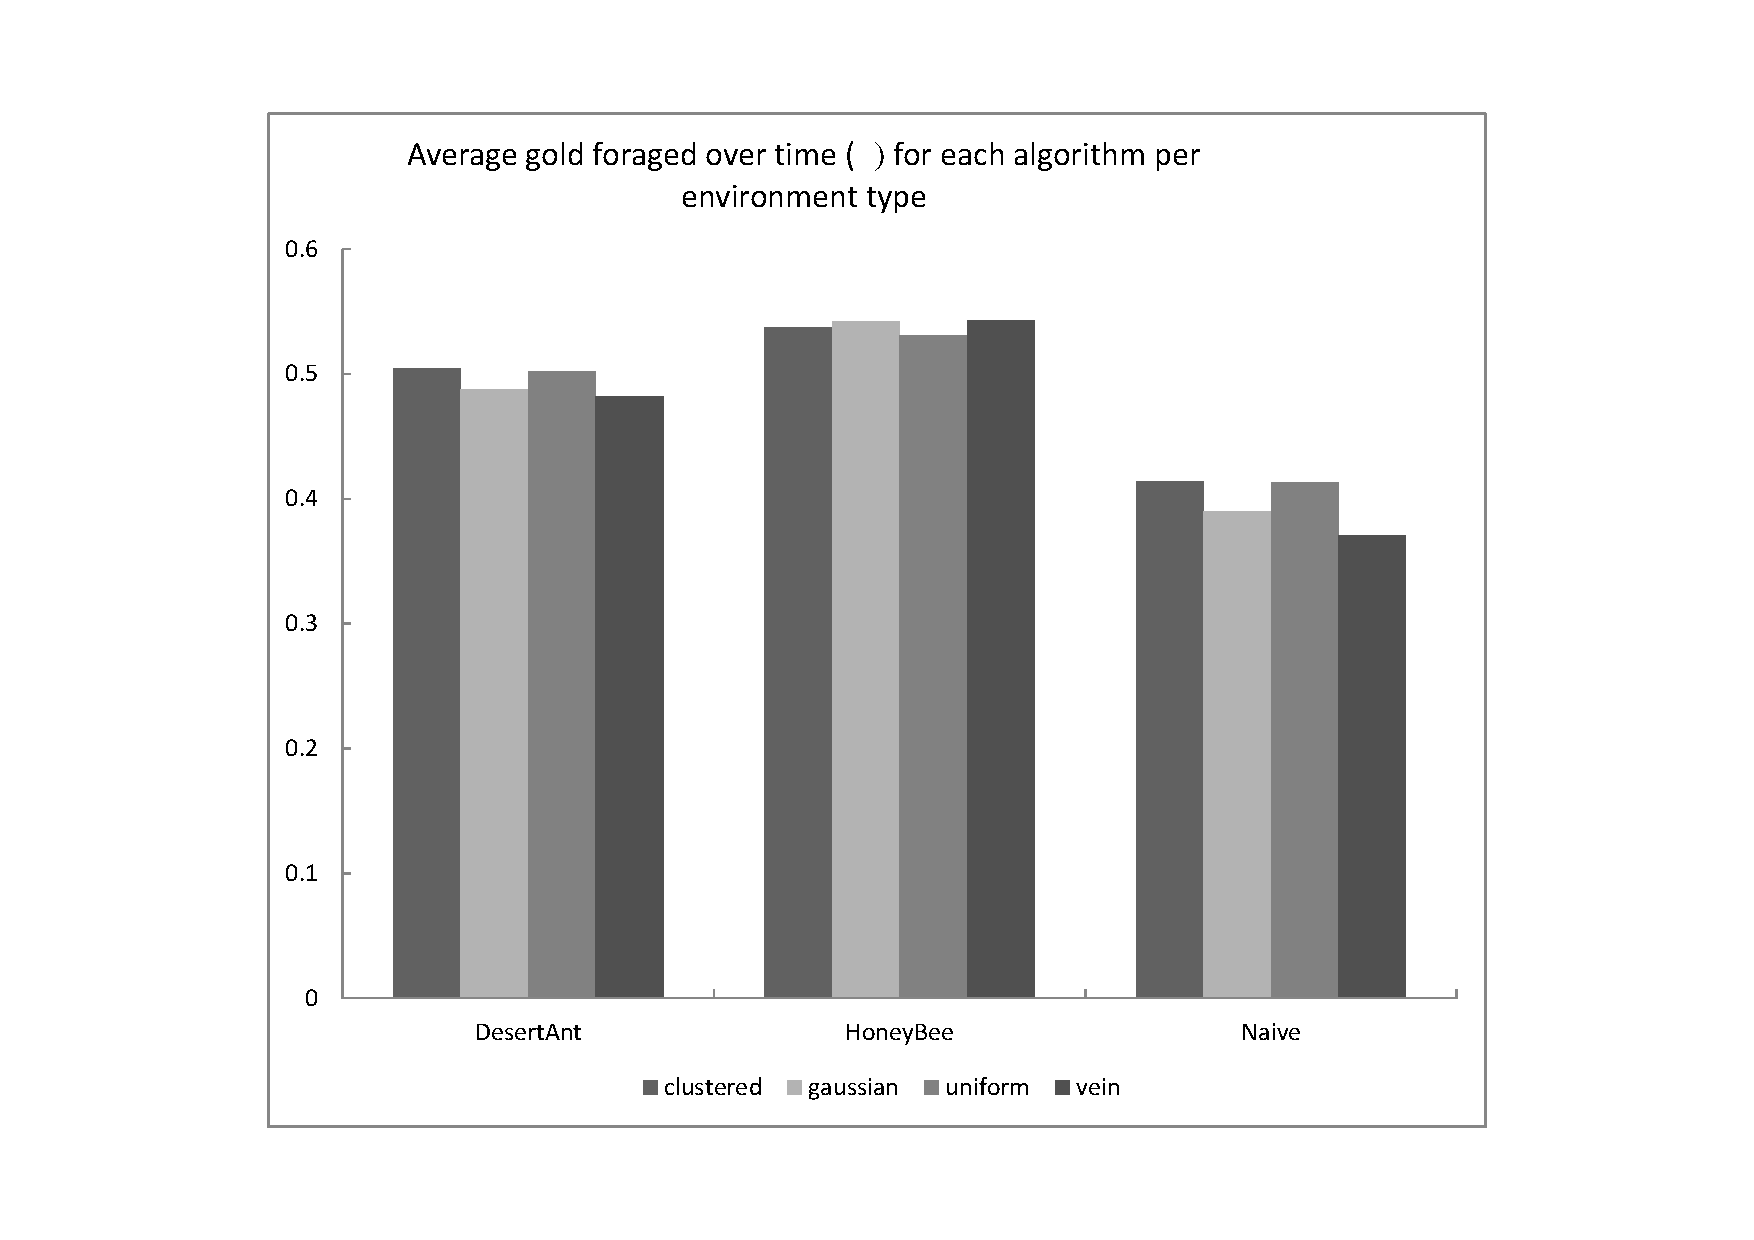
\includegraphics[width=\textwidth]{chapters/chapter6/graphs/gold_environment.pdf}
\caption{Prioritized items over time per environment type for each algorithm}
\label{environmentgoldplot}
\end{figure}

\begin{figure}[!htb]
\centering
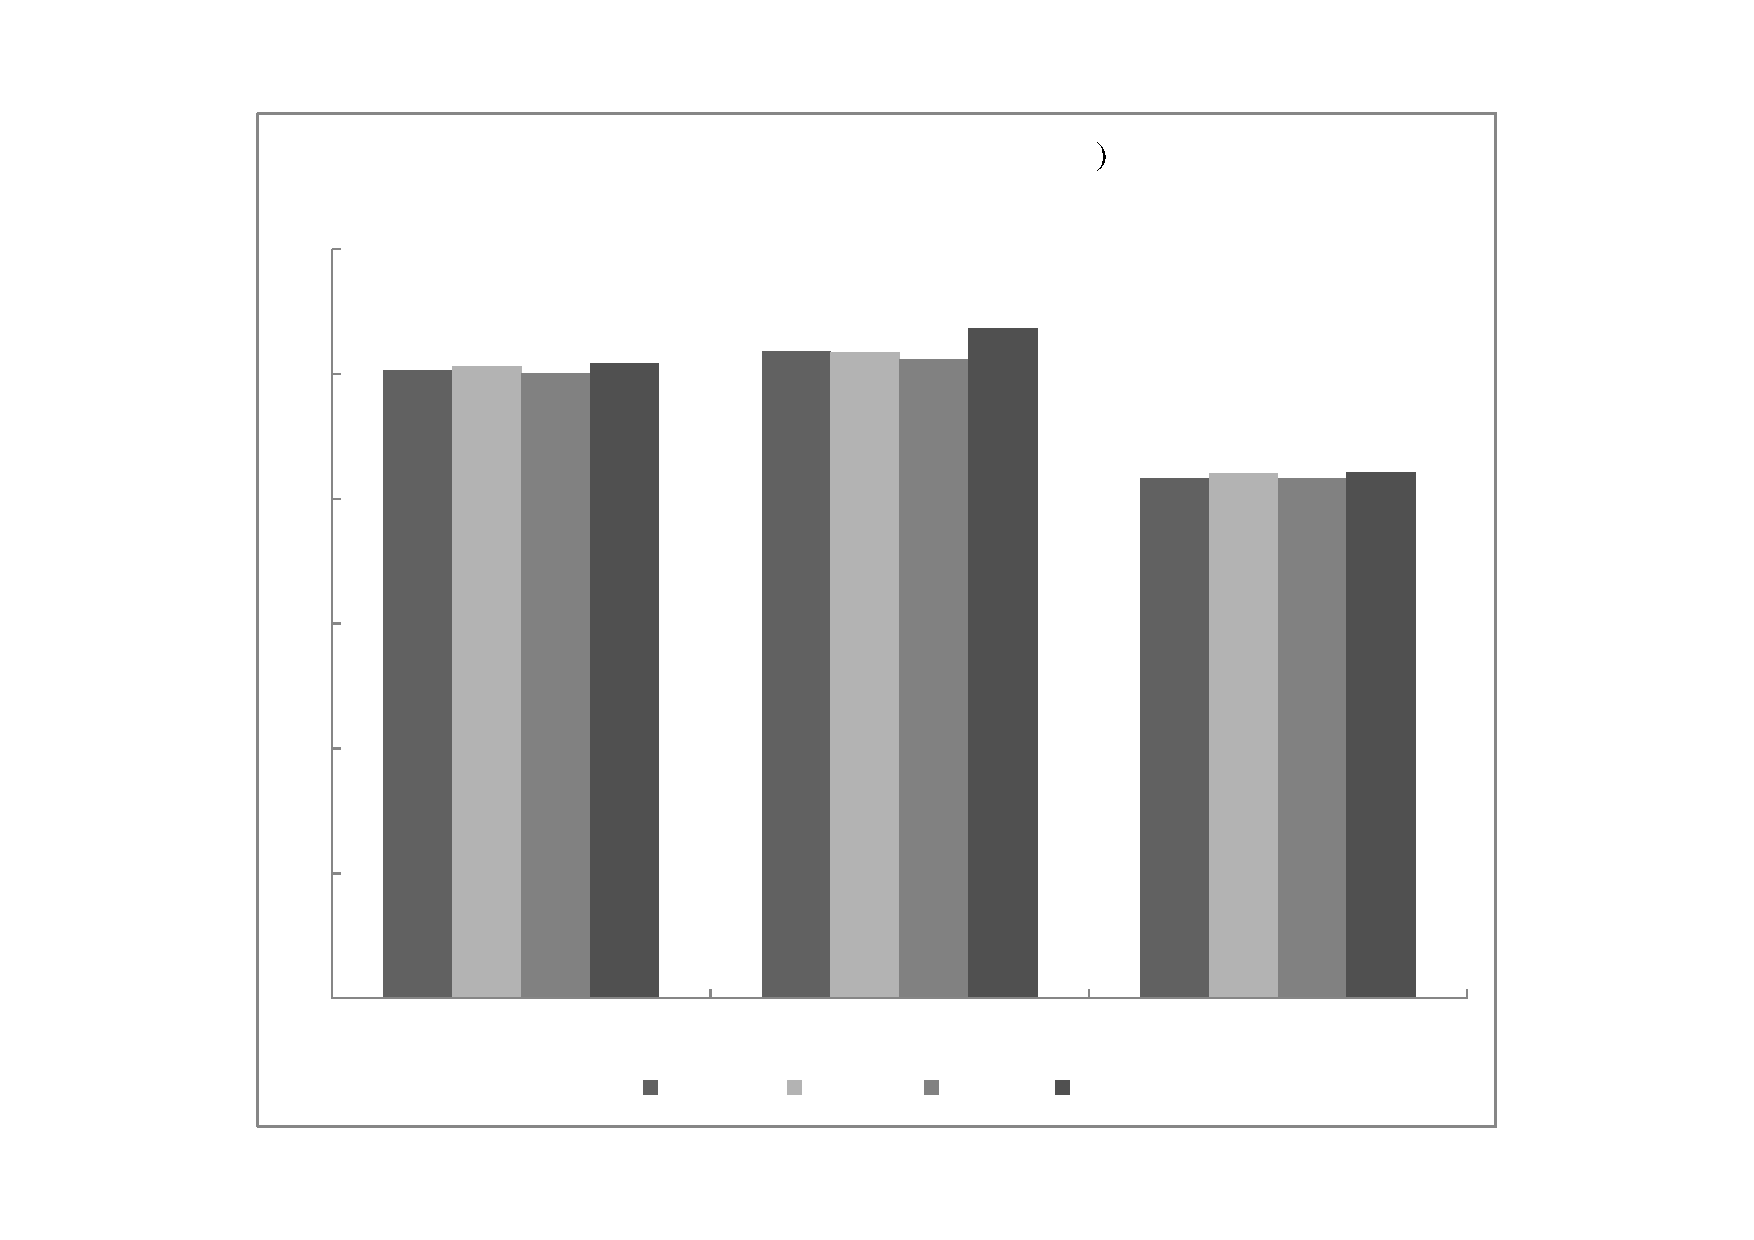
\includegraphics[width=\textwidth]{chapters/chapter6/graphs/waste_environment.pdf}
\caption{Non-prioritized items over time per environment type for each algorithm}
\label{environmentgoldplot}
\end{figure}

%Discussion
Although the Mann-whitney U tests show that their is a significant difference, from the graphs and tables, the averages show that the significant difference is quite small. This could mean 1 or a few things
\begin{enumerate}
	\item The environments that have been generated are not very different or of good quality.
	\item The algorithms do not have a particular preference to a specific environment type, or can't exploit characteristics of specific environment types particularly well.
\end{enumerate}

That being said, the tests still indicate a significant difference, the magnitude of which may be increased by better algorithm quality. Starting with the na\"ive algorithm, the results are mostly as would be expected. The algorithm achieves best performance on the uniform and clustered environments. These environments, particularly the uniform environments, would not require one to move past large areas of non-prioritized items. What is interesting is that the na\"ive algorithm performed a little better on the clustered environments. This could plausibly be attributed to the fact that the clustered environments would have empty paths between clusters created by the luma faita based generation algorithm. The gaussian and vein environments are harder for the na\"ive algorithm, since the environment would involve moving past large areas of non-prioritized items to get to the prioritized items. This could also be due to the inability of the algorithm to exploit good areas of the search space via memory-based techniques or communication.

The desert and algorithm shows similar differences, although with smaller differences between algorithm type. The similarity between the na\"ive and desert ants environment type performance suggests that it is not the ability of an algorithm to exploit good areas of the search space but rather the inability to move past large areas of non-prioritized items to get to prioritized items.

The honey bee algorithm has very small differences between algorithm type, highlighting the honey bee algorithm's flexibility. The algorithm performed better on the vein and gaussian environments than on the uniform and clustered environments. This suggests that the division of labour may be able to adapt well to current dominant item type in the area then adequately switch to a changed dominant item type.
%TODO: Talk about why performs worse on clustered and uniform.

What is most interesting is that the honey bee algorithm still performed better than desert ant and na\"ive foraging on the uniform environments. Communication of good locations is unlikely to benefit in the uniform environments, nor is memory of prior locations, since there is no concentration of items. So the most likely attribute of the honey bee algorithm is the division of labour. If the division of labour between items types is perfect then the algorithm would likely outperform the algorithm which does not have a perfect division of labour. This would be because if there are too many robots foraging the non-prioritized items and not enough prioritized items, then robots are possibly wasting time bouncing off items which are not of their type. %TODO: Would be cool to show this somewhere. 

%Talk about why desert ant is better than naive in uniform environments
Desert ant out performs na\"ive algorithm as well in uniform environments. As stated previously, this result is unlikely to be attributed to the memorization of prior locations since algorithms are uniformly distributed. The most possible reason for this may be since less random walk occurs. If an item is found by the desert ant agent, next time the robot wants to find an item it will attempt to return directly to the prior location. The fact that there isn't an item exactly where the desert ant was is inconsequential. Since the environment is uniformly distributed, there is a high chance that there is an item nearby. This would become particularly evident when the agents have cleared the areas closer to the sink and have to go deeper into the environment to find items. The desert ant algorithm would first move directly to the old location, without random walk which may turn back on itself and if no item exists, the robot will start the random walk again. In general, for both honey bee and desert ant, the fact that more direct routes to items occurred seems to have improved performance. 

%Talk about the fact honey bee foraged more waste on the vein environments.   (in order to get to the trapped gold)
To further enforce the fact that the honey bee division of labour was effective, if one looks at the non-prioritized items over time, one will notice that the non-prioritized items over time is much higher than the others. This can possibly be attributed to the fact that the robots would have to forage large amount of non-prioritized items first before getting to the prioritized items.

%Discuss the waste over time. 
Looking more at the non-prioritized items over time, there is evidence with na\"ive and desert ant algorithms, on the environment types that they found difficult to forage prioritized items on, foraged more non-prioritized showing, once again the benefit of having division of labour. %TODO: Explain better. 

\section{Robustness}
\label{results:robustness}

%Intro discussion

\subsection{Environmental Complexity}
\label{results:environmentcomplexity}
%How are the algorithms affected by changes in object quantity - more objects, very high waste  

%Mann-WHitney U & average
%Graphs comparing performance of environmental types

\begin{table} [h]
     \caption{Prioritized items over time over Object Percentage in Environment  for each algorithm}
     \label{ratio}
	\centering
	\footnotesize
	\begin{tabular} {|l|l|l|l|}
\hline
$p$ & Naive & DesertAnt & HoneyBee \\
\hline
0.05 & 0.58576 (0.397434)  & 0.709257 (0.370191)  & 0.724892 (0.331663)  \\
0.2 & 0.445301 (0.400194)  & 0.55749 (0.396821)  & 0.601527 (0.374943)  \\
0.5 & 0.34856 (0.3778)  & 0.441694 (0.395469)  & 0.494143 (0.388125)  \\
0.7 & 0.315063 (0.368166)  & 0.396919 (0.389359)  & 0.451818 (0.388338)  \\
0.9 & 0.290859 (0.360364)  & 0.365705 (0.383365)  & 0.418788 (0.38623)  \\
\hline
\end{tabular}

\end{table}

\begin{figure}[!htb]
\centering
\resizebox{\textwidth}{!}{% GNUPLOT: LaTeX picture with Postscript
\begingroup
  \makeatletter
  \providecommand\color[2][]{%
    \GenericError{(gnuplot) \space\space\space\@spaces}{%
      Package color not loaded in conjunction with
      terminal option `colourtext'%
    }{See the gnuplot documentation for explanation.%
    }{Either use 'blacktext' in gnuplot or load the package
      color.sty in LaTeX.}%
    \renewcommand\color[2][]{}%
  }%
  \providecommand\includegraphics[2][]{%
    \GenericError{(gnuplot) \space\space\space\@spaces}{%
      Package graphicx or graphics not loaded%
    }{See the gnuplot documentation for explanation.%
    }{The gnuplot epslatex terminal needs graphicx.sty or graphics.sty.}%
    \renewcommand\includegraphics[2][]{}%
  }%
  \providecommand\rotatebox[2]{#2}%
  \@ifundefined{ifGPcolor}{%
    \newif\ifGPcolor
    \GPcolorfalse
  }{}%
  \@ifundefined{ifGPblacktext}{%
    \newif\ifGPblacktext
    \GPblacktexttrue
  }{}%
  % define a \g@addto@macro without @ in the name:
  \let\gplgaddtomacro\g@addto@macro
  % define empty templates for all commands taking text:
  \gdef\gplbacktext{}%
  \gdef\gplfronttext{}%
  \makeatother
  \ifGPblacktext
    % no textcolor at all
    \def\colorrgb#1{}%
    \def\colorgray#1{}%
  \else
    % gray or color?
    \ifGPcolor
      \def\colorrgb#1{\color[rgb]{#1}}%
      \def\colorgray#1{\color[gray]{#1}}%
      \expandafter\def\csname LTw\endcsname{\color{white}}%
      \expandafter\def\csname LTb\endcsname{\color{black}}%
      \expandafter\def\csname LTa\endcsname{\color{black}}%
      \expandafter\def\csname LT0\endcsname{\color[rgb]{1,0,0}}%
      \expandafter\def\csname LT1\endcsname{\color[rgb]{0,1,0}}%
      \expandafter\def\csname LT2\endcsname{\color[rgb]{0,0,1}}%
      \expandafter\def\csname LT3\endcsname{\color[rgb]{1,0,1}}%
      \expandafter\def\csname LT4\endcsname{\color[rgb]{0,1,1}}%
      \expandafter\def\csname LT5\endcsname{\color[rgb]{1,1,0}}%
      \expandafter\def\csname LT6\endcsname{\color[rgb]{0,0,0}}%
      \expandafter\def\csname LT7\endcsname{\color[rgb]{1,0.3,0}}%
      \expandafter\def\csname LT8\endcsname{\color[rgb]{0.5,0.5,0.5}}%
    \else
      % gray
      \def\colorrgb#1{\color{black}}%
      \def\colorgray#1{\color[gray]{#1}}%
      \expandafter\def\csname LTw\endcsname{\color{white}}%
      \expandafter\def\csname LTb\endcsname{\color{black}}%
      \expandafter\def\csname LTa\endcsname{\color{black}}%
      \expandafter\def\csname LT0\endcsname{\color{black}}%
      \expandafter\def\csname LT1\endcsname{\color{black}}%
      \expandafter\def\csname LT2\endcsname{\color{black}}%
      \expandafter\def\csname LT3\endcsname{\color{black}}%
      \expandafter\def\csname LT4\endcsname{\color{black}}%
      \expandafter\def\csname LT5\endcsname{\color{black}}%
      \expandafter\def\csname LT6\endcsname{\color{black}}%
      \expandafter\def\csname LT7\endcsname{\color{black}}%
      \expandafter\def\csname LT8\endcsname{\color{black}}%
    \fi
  \fi
  \setlength{\unitlength}{0.0500bp}%
  \begin{picture}(7200.00,5040.00)%
    \gplgaddtomacro\gplbacktext{%
      \csname LTb\endcsname%
      \put(1078,704){\makebox(0,0)[r]{\strut{} 0.25}}%
      \put(1078,1071){\makebox(0,0)[r]{\strut{} 0.3}}%
      \put(1078,1439){\makebox(0,0)[r]{\strut{} 0.35}}%
      \put(1078,1806){\makebox(0,0)[r]{\strut{} 0.4}}%
      \put(1078,2174){\makebox(0,0)[r]{\strut{} 0.45}}%
      \put(1078,2541){\makebox(0,0)[r]{\strut{} 0.5}}%
      \put(1078,2909){\makebox(0,0)[r]{\strut{} 0.55}}%
      \put(1078,3276){\makebox(0,0)[r]{\strut{} 0.6}}%
      \put(1078,3644){\makebox(0,0)[r]{\strut{} 0.65}}%
      \put(1078,4012){\makebox(0,0)[r]{\strut{} 0.7}}%
      \put(1078,4379){\makebox(0,0)[r]{\strut{} 0.75}}%
      \put(1210,484){\makebox(0,0){\strut{} 0}}%
      \put(1831,484){\makebox(0,0){\strut{} 0.1}}%
      \put(2453,484){\makebox(0,0){\strut{} 0.2}}%
      \put(3074,484){\makebox(0,0){\strut{} 0.3}}%
      \put(3696,484){\makebox(0,0){\strut{} 0.4}}%
      \put(4317,484){\makebox(0,0){\strut{} 0.5}}%
      \put(4939,484){\makebox(0,0){\strut{} 0.6}}%
      \put(5560,484){\makebox(0,0){\strut{} 0.7}}%
      \put(6182,484){\makebox(0,0){\strut{} 0.8}}%
      \put(6803,484){\makebox(0,0){\strut{} 0.9}}%
      \put(176,2541){\rotatebox{-270}{\makebox(0,0){\strut{}Prioritized items over time ($\sigma$)}}}%
      \put(4006,154){\makebox(0,0){\strut{}Amount of Objects ($p$)}}%
      \put(4006,4709){\makebox(0,0){\strut{}Prioritized items over time for each algorithm over item density}}%
    }%
    \gplgaddtomacro\gplfronttext{%
      \csname LTb\endcsname%
      \put(5816,4206){\makebox(0,0)[r]{\strut{}Na\"ive}}%
      \csname LTb\endcsname%
      \put(5816,3986){\makebox(0,0)[r]{\strut{}Desert Ant}}%
      \csname LTb\endcsname%
      \put(5816,3766){\makebox(0,0)[r]{\strut{}Honey Bee}}%
    }%
    \gplbacktext
    \put(0,0){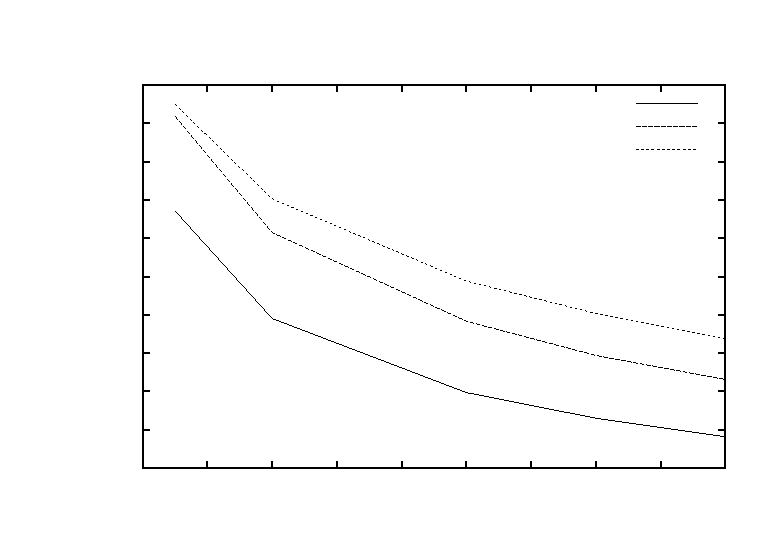
\includegraphics{chapters/chapter6/graphs/gold_objects}}%
    \gplfronttext
  \end{picture}%
\endgroup
}
\caption{Prioritized items over time over Object Percentage in Environment  for each algorithm}
\label{objectgoldplot}
\end{figure}


\begin{figure}[!htb]
\centering
\resizebox{\textwidth}{!}{% GNUPLOT: LaTeX picture with Postscript
\begingroup
  \makeatletter
  \providecommand\color[2][]{%
    \GenericError{(gnuplot) \space\space\space\@spaces}{%
      Package color not loaded in conjunction with
      terminal option `colourtext'%
    }{See the gnuplot documentation for explanation.%
    }{Either use 'blacktext' in gnuplot or load the package
      color.sty in LaTeX.}%
    \renewcommand\color[2][]{}%
  }%
  \providecommand\includegraphics[2][]{%
    \GenericError{(gnuplot) \space\space\space\@spaces}{%
      Package graphicx or graphics not loaded%
    }{See the gnuplot documentation for explanation.%
    }{The gnuplot epslatex terminal needs graphicx.sty or graphics.sty.}%
    \renewcommand\includegraphics[2][]{}%
  }%
  \providecommand\rotatebox[2]{#2}%
  \@ifundefined{ifGPcolor}{%
    \newif\ifGPcolor
    \GPcolorfalse
  }{}%
  \@ifundefined{ifGPblacktext}{%
    \newif\ifGPblacktext
    \GPblacktexttrue
  }{}%
  % define a \g@addto@macro without @ in the name:
  \let\gplgaddtomacro\g@addto@macro
  % define empty templates for all commands taking text:
  \gdef\gplbacktext{}%
  \gdef\gplfronttext{}%
  \makeatother
  \ifGPblacktext
    % no textcolor at all
    \def\colorrgb#1{}%
    \def\colorgray#1{}%
  \else
    % gray or color?
    \ifGPcolor
      \def\colorrgb#1{\color[rgb]{#1}}%
      \def\colorgray#1{\color[gray]{#1}}%
      \expandafter\def\csname LTw\endcsname{\color{white}}%
      \expandafter\def\csname LTb\endcsname{\color{black}}%
      \expandafter\def\csname LTa\endcsname{\color{black}}%
      \expandafter\def\csname LT0\endcsname{\color[rgb]{1,0,0}}%
      \expandafter\def\csname LT1\endcsname{\color[rgb]{0,1,0}}%
      \expandafter\def\csname LT2\endcsname{\color[rgb]{0,0,1}}%
      \expandafter\def\csname LT3\endcsname{\color[rgb]{1,0,1}}%
      \expandafter\def\csname LT4\endcsname{\color[rgb]{0,1,1}}%
      \expandafter\def\csname LT5\endcsname{\color[rgb]{1,1,0}}%
      \expandafter\def\csname LT6\endcsname{\color[rgb]{0,0,0}}%
      \expandafter\def\csname LT7\endcsname{\color[rgb]{1,0.3,0}}%
      \expandafter\def\csname LT8\endcsname{\color[rgb]{0.5,0.5,0.5}}%
    \else
      % gray
      \def\colorrgb#1{\color{black}}%
      \def\colorgray#1{\color[gray]{#1}}%
      \expandafter\def\csname LTw\endcsname{\color{white}}%
      \expandafter\def\csname LTb\endcsname{\color{black}}%
      \expandafter\def\csname LTa\endcsname{\color{black}}%
      \expandafter\def\csname LT0\endcsname{\color{black}}%
      \expandafter\def\csname LT1\endcsname{\color{black}}%
      \expandafter\def\csname LT2\endcsname{\color{black}}%
      \expandafter\def\csname LT3\endcsname{\color{black}}%
      \expandafter\def\csname LT4\endcsname{\color{black}}%
      \expandafter\def\csname LT5\endcsname{\color{black}}%
      \expandafter\def\csname LT6\endcsname{\color{black}}%
      \expandafter\def\csname LT7\endcsname{\color{black}}%
      \expandafter\def\csname LT8\endcsname{\color{black}}%
    \fi
  \fi
  \setlength{\unitlength}{0.0500bp}%
  \begin{picture}(7200.00,5040.00)%
    \gplgaddtomacro\gplbacktext{%
      \csname LTb\endcsname%
      \put(946,704){\makebox(0,0)[r]{\strut{} 0.3}}%
      \put(946,1229){\makebox(0,0)[r]{\strut{} 0.4}}%
      \put(946,1754){\makebox(0,0)[r]{\strut{} 0.5}}%
      \put(946,2279){\makebox(0,0)[r]{\strut{} 0.6}}%
      \put(946,2804){\makebox(0,0)[r]{\strut{} 0.7}}%
      \put(946,3329){\makebox(0,0)[r]{\strut{} 0.8}}%
      \put(946,3854){\makebox(0,0)[r]{\strut{} 0.9}}%
      \put(946,4379){\makebox(0,0)[r]{\strut{} 1}}%
      \put(1078,484){\makebox(0,0){\strut{} 0}}%
      \put(2223,484){\makebox(0,0){\strut{} 0.2}}%
      \put(3368,484){\makebox(0,0){\strut{} 0.4}}%
      \put(4513,484){\makebox(0,0){\strut{} 0.6}}%
      \put(5658,484){\makebox(0,0){\strut{} 0.8}}%
      \put(6803,484){\makebox(0,0){\strut{} 1}}%
      \put(176,2541){\rotatebox{-270}{\makebox(0,0){\strut{}Non-prioritized items over time ($\sigma$)}}}%
      \put(3940,154){\makebox(0,0){\strut{}Amount of Objects ($p$)}}%
      \put(3940,4709){\makebox(0,0){\strut{}Non-prioritized items over time for each algorithm over object percentages}}%
    }%
    \gplgaddtomacro\gplfronttext{%
      \csname LTb\endcsname%
      \put(5816,4206){\makebox(0,0)[r]{\strut{}Na\"ive}}%
      \csname LTb\endcsname%
      \put(5816,3986){\makebox(0,0)[r]{\strut{}Desert Ant}}%
      \csname LTb\endcsname%
      \put(5816,3766){\makebox(0,0)[r]{\strut{}Honey Bee}}%
    }%
    \gplbacktext
    \put(0,0){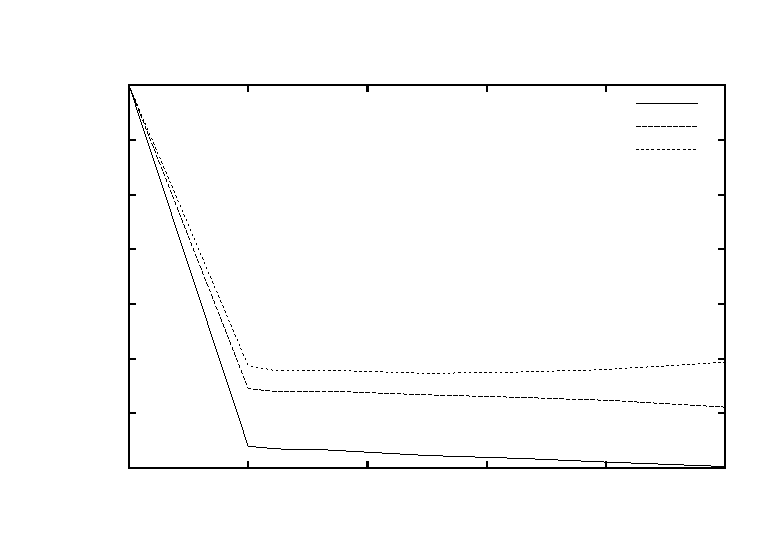
\includegraphics{chapters/chapter6/graphs/waste_objects}}%
    \gplfronttext
  \end{picture}%
\endgroup
}
\caption{Non-prioritized items over time over Object Percentage in Environment for each algorithm}
\label{objectgoldplot}
\end{figure}

%Discussion
All algorithms are shown to degrade quite heavily as the number of objects increases, but that is plausibly because there was a limit on simulation time. To adequately analyse the performance over objects one would have to allow more time to simulations. 

\subsection{Division}
\label{results:division}

%Desert Ant algorithm
%Has optimal configuration that is unaffected by ratio. 
%Honey bee: 
%Does the division of labour benefit the algorithm.
%No, not in static context? Why? 
%Possibly in a dynamic context? Discussion. Future work

\begin{figure}[!htb]
\centering
\resizebox{\textwidth}{!}{% GNUPLOT: LaTeX picture with Postscript
\begingroup
  \makeatletter
  \providecommand\color[2][]{%
    \GenericError{(gnuplot) \space\space\space\@spaces}{%
      Package color not loaded in conjunction with
      terminal option `colourtext'%
    }{See the gnuplot documentation for explanation.%
    }{Either use 'blacktext' in gnuplot or load the package
      color.sty in LaTeX.}%
    \renewcommand\color[2][]{}%
  }%
  \providecommand\includegraphics[2][]{%
    \GenericError{(gnuplot) \space\space\space\@spaces}{%
      Package graphicx or graphics not loaded%
    }{See the gnuplot documentation for explanation.%
    }{The gnuplot epslatex terminal needs graphicx.sty or graphics.sty.}%
    \renewcommand\includegraphics[2][]{}%
  }%
  \providecommand\rotatebox[2]{#2}%
  \@ifundefined{ifGPcolor}{%
    \newif\ifGPcolor
    \GPcolorfalse
  }{}%
  \@ifundefined{ifGPblacktext}{%
    \newif\ifGPblacktext
    \GPblacktexttrue
  }{}%
  % define a \g@addto@macro without @ in the name:
  \let\gplgaddtomacro\g@addto@macro
  % define empty templates for all commands taking text:
  \gdef\gplbacktext{}%
  \gdef\gplfronttext{}%
  \makeatother
  \ifGPblacktext
    % no textcolor at all
    \def\colorrgb#1{}%
    \def\colorgray#1{}%
  \else
    % gray or color?
    \ifGPcolor
      \def\colorrgb#1{\color[rgb]{#1}}%
      \def\colorgray#1{\color[gray]{#1}}%
      \expandafter\def\csname LTw\endcsname{\color{white}}%
      \expandafter\def\csname LTb\endcsname{\color{black}}%
      \expandafter\def\csname LTa\endcsname{\color{black}}%
      \expandafter\def\csname LT0\endcsname{\color[rgb]{1,0,0}}%
      \expandafter\def\csname LT1\endcsname{\color[rgb]{0,1,0}}%
      \expandafter\def\csname LT2\endcsname{\color[rgb]{0,0,1}}%
      \expandafter\def\csname LT3\endcsname{\color[rgb]{1,0,1}}%
      \expandafter\def\csname LT4\endcsname{\color[rgb]{0,1,1}}%
      \expandafter\def\csname LT5\endcsname{\color[rgb]{1,1,0}}%
      \expandafter\def\csname LT6\endcsname{\color[rgb]{0,0,0}}%
      \expandafter\def\csname LT7\endcsname{\color[rgb]{1,0.3,0}}%
      \expandafter\def\csname LT8\endcsname{\color[rgb]{0.5,0.5,0.5}}%
    \else
      % gray
      \def\colorrgb#1{\color{black}}%
      \def\colorgray#1{\color[gray]{#1}}%
      \expandafter\def\csname LTw\endcsname{\color{white}}%
      \expandafter\def\csname LTb\endcsname{\color{black}}%
      \expandafter\def\csname LTa\endcsname{\color{black}}%
      \expandafter\def\csname LT0\endcsname{\color{black}}%
      \expandafter\def\csname LT1\endcsname{\color{black}}%
      \expandafter\def\csname LT2\endcsname{\color{black}}%
      \expandafter\def\csname LT3\endcsname{\color{black}}%
      \expandafter\def\csname LT4\endcsname{\color{black}}%
      \expandafter\def\csname LT5\endcsname{\color{black}}%
      \expandafter\def\csname LT6\endcsname{\color{black}}%
      \expandafter\def\csname LT7\endcsname{\color{black}}%
      \expandafter\def\csname LT8\endcsname{\color{black}}%
    \fi
  \fi
  \setlength{\unitlength}{0.0500bp}%
  \begin{picture}(7200.00,5040.00)%
    \gplgaddtomacro\gplbacktext{%
      \csname LTb\endcsname%
      \put(1078,704){\makebox(0,0)[r]{\strut{} 0.1}}%
      \put(1078,1072){\makebox(0,0)[r]{\strut{} 0.15}}%
      \put(1078,1439){\makebox(0,0)[r]{\strut{} 0.2}}%
      \put(1078,1806){\makebox(0,0)[r]{\strut{} 0.25}}%
      \put(1078,2174){\makebox(0,0)[r]{\strut{} 0.3}}%
      \put(1078,2541){\makebox(0,0)[r]{\strut{} 0.35}}%
      \put(1078,2909){\makebox(0,0)[r]{\strut{} 0.4}}%
      \put(1078,3276){\makebox(0,0)[r]{\strut{} 0.45}}%
      \put(1078,3644){\makebox(0,0)[r]{\strut{} 0.5}}%
      \put(1078,4011){\makebox(0,0)[r]{\strut{} 0.55}}%
      \put(1078,4379){\makebox(0,0)[r]{\strut{} 0.6}}%
      \put(1210,484){\makebox(0,0){\strut{} 0}}%
      \put(2329,484){\makebox(0,0){\strut{} 0.2}}%
      \put(3447,484){\makebox(0,0){\strut{} 0.4}}%
      \put(4566,484){\makebox(0,0){\strut{} 0.6}}%
      \put(5684,484){\makebox(0,0){\strut{} 0.8}}%
      \put(6803,484){\makebox(0,0){\strut{} 1}}%
      \put(176,2541){\rotatebox{-270}{\makebox(0,0){\strut{}Prioritized items over time ($\sigma$)}}}%
      \put(4006,154){\makebox(0,0){\strut{}Robot Type Ratio ($r$)}}%
      \put(4006,4709){\makebox(0,0){\strut{}Prioritized items over time for each algorithm for robot type ratios}}%
    }%
    \gplgaddtomacro\gplfronttext{%
      \csname LTb\endcsname%
      \put(5816,4206){\makebox(0,0)[r]{\strut{}Na\"ive}}%
      \csname LTb\endcsname%
      \put(5816,3986){\makebox(0,0)[r]{\strut{}Desert Ant}}%
      \csname LTb\endcsname%
      \put(5816,3766){\makebox(0,0)[r]{\strut{}Honey Bee}}%
    }%
    \gplbacktext
    \put(0,0){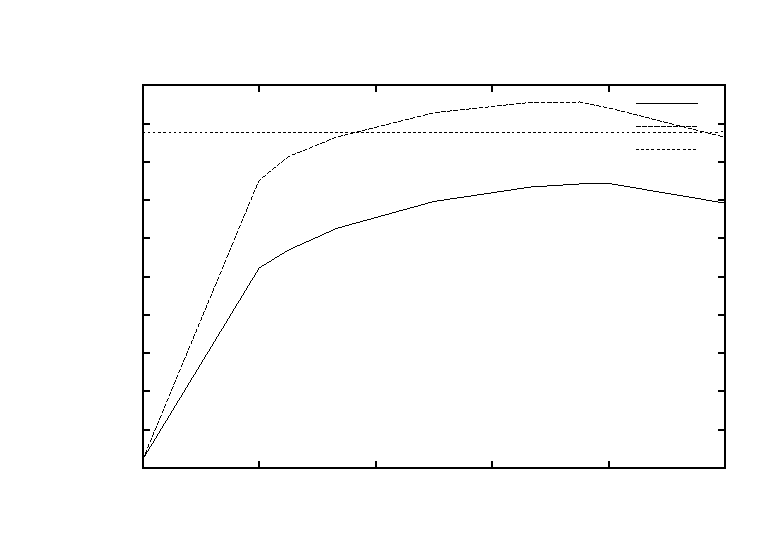
\includegraphics{chapters/chapter6/graphs/gold_division}}%
    \gplfronttext
  \end{picture}%
\endgroup
}
\caption{Prioritized items over time over ratio of robots in environment for each algorithm }
\label{divisiongoldplot}
\end{figure}


\begin{figure}[!htb]
\centering
\resizebox{\textwidth}{!}{% GNUPLOT: LaTeX picture with Postscript
\begingroup
  \makeatletter
  \providecommand\color[2][]{%
    \GenericError{(gnuplot) \space\space\space\@spaces}{%
      Package color not loaded in conjunction with
      terminal option `colourtext'%
    }{See the gnuplot documentation for explanation.%
    }{Either use 'blacktext' in gnuplot or load the package
      color.sty in LaTeX.}%
    \renewcommand\color[2][]{}%
  }%
  \providecommand\includegraphics[2][]{%
    \GenericError{(gnuplot) \space\space\space\@spaces}{%
      Package graphicx or graphics not loaded%
    }{See the gnuplot documentation for explanation.%
    }{The gnuplot epslatex terminal needs graphicx.sty or graphics.sty.}%
    \renewcommand\includegraphics[2][]{}%
  }%
  \providecommand\rotatebox[2]{#2}%
  \@ifundefined{ifGPcolor}{%
    \newif\ifGPcolor
    \GPcolorfalse
  }{}%
  \@ifundefined{ifGPblacktext}{%
    \newif\ifGPblacktext
    \GPblacktexttrue
  }{}%
  % define a \g@addto@macro without @ in the name:
  \let\gplgaddtomacro\g@addto@macro
  % define empty templates for all commands taking text:
  \gdef\gplbacktext{}%
  \gdef\gplfronttext{}%
  \makeatother
  \ifGPblacktext
    % no textcolor at all
    \def\colorrgb#1{}%
    \def\colorgray#1{}%
  \else
    % gray or color?
    \ifGPcolor
      \def\colorrgb#1{\color[rgb]{#1}}%
      \def\colorgray#1{\color[gray]{#1}}%
      \expandafter\def\csname LTw\endcsname{\color{white}}%
      \expandafter\def\csname LTb\endcsname{\color{black}}%
      \expandafter\def\csname LTa\endcsname{\color{black}}%
      \expandafter\def\csname LT0\endcsname{\color[rgb]{1,0,0}}%
      \expandafter\def\csname LT1\endcsname{\color[rgb]{0,1,0}}%
      \expandafter\def\csname LT2\endcsname{\color[rgb]{0,0,1}}%
      \expandafter\def\csname LT3\endcsname{\color[rgb]{1,0,1}}%
      \expandafter\def\csname LT4\endcsname{\color[rgb]{0,1,1}}%
      \expandafter\def\csname LT5\endcsname{\color[rgb]{1,1,0}}%
      \expandafter\def\csname LT6\endcsname{\color[rgb]{0,0,0}}%
      \expandafter\def\csname LT7\endcsname{\color[rgb]{1,0.3,0}}%
      \expandafter\def\csname LT8\endcsname{\color[rgb]{0.5,0.5,0.5}}%
    \else
      % gray
      \def\colorrgb#1{\color{black}}%
      \def\colorgray#1{\color[gray]{#1}}%
      \expandafter\def\csname LTw\endcsname{\color{white}}%
      \expandafter\def\csname LTb\endcsname{\color{black}}%
      \expandafter\def\csname LTa\endcsname{\color{black}}%
      \expandafter\def\csname LT0\endcsname{\color{black}}%
      \expandafter\def\csname LT1\endcsname{\color{black}}%
      \expandafter\def\csname LT2\endcsname{\color{black}}%
      \expandafter\def\csname LT3\endcsname{\color{black}}%
      \expandafter\def\csname LT4\endcsname{\color{black}}%
      \expandafter\def\csname LT5\endcsname{\color{black}}%
      \expandafter\def\csname LT6\endcsname{\color{black}}%
      \expandafter\def\csname LT7\endcsname{\color{black}}%
      \expandafter\def\csname LT8\endcsname{\color{black}}%
    \fi
  \fi
  \setlength{\unitlength}{0.0500bp}%
  \begin{picture}(7200.00,5040.00)%
    \gplgaddtomacro\gplbacktext{%
      \csname LTb\endcsname%
      \put(1078,704){\makebox(0,0)[r]{\strut{} 0.1}}%
      \put(1078,1072){\makebox(0,0)[r]{\strut{} 0.15}}%
      \put(1078,1439){\makebox(0,0)[r]{\strut{} 0.2}}%
      \put(1078,1806){\makebox(0,0)[r]{\strut{} 0.25}}%
      \put(1078,2174){\makebox(0,0)[r]{\strut{} 0.3}}%
      \put(1078,2541){\makebox(0,0)[r]{\strut{} 0.35}}%
      \put(1078,2909){\makebox(0,0)[r]{\strut{} 0.4}}%
      \put(1078,3276){\makebox(0,0)[r]{\strut{} 0.45}}%
      \put(1078,3644){\makebox(0,0)[r]{\strut{} 0.5}}%
      \put(1078,4011){\makebox(0,0)[r]{\strut{} 0.55}}%
      \put(1078,4379){\makebox(0,0)[r]{\strut{} 0.6}}%
      \put(1210,484){\makebox(0,0){\strut{} 0}}%
      \put(2329,484){\makebox(0,0){\strut{} 0.2}}%
      \put(3447,484){\makebox(0,0){\strut{} 0.4}}%
      \put(4566,484){\makebox(0,0){\strut{} 0.6}}%
      \put(5684,484){\makebox(0,0){\strut{} 0.8}}%
      \put(6803,484){\makebox(0,0){\strut{} 1}}%
      \put(176,2541){\rotatebox{-270}{\makebox(0,0){\strut{}Non-prioritized items over time ($\tau$)}}}%
      \put(4006,154){\makebox(0,0){\strut{}Robot Specialization Ratio($\tau$)}}%
      \put(4006,4709){\makebox(0,0){\strut{}Non-prioritized items over time for each algorithm for robot specialization ratios}}%
    }%
    \gplgaddtomacro\gplfronttext{%
      \csname LTb\endcsname%
      \put(5816,4206){\makebox(0,0)[r]{\strut{}Na\"ive}}%
      \csname LTb\endcsname%
      \put(5816,3986){\makebox(0,0)[r]{\strut{}Desert Ant}}%
      \csname LTb\endcsname%
      \put(5816,3766){\makebox(0,0)[r]{\strut{}Honey Bee}}%
    }%
    \gplbacktext
    \put(0,0){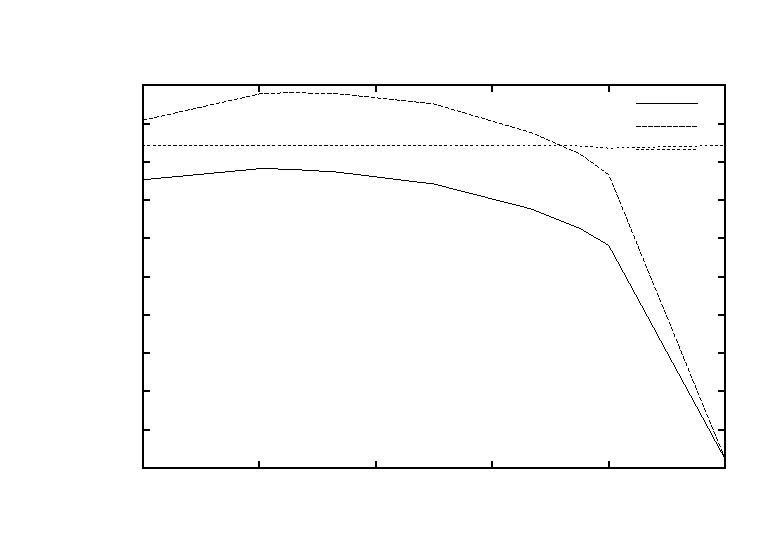
\includegraphics{chapters/chapter6/graphs/waste_division}}%
    \gplfronttext
  \end{picture}%
\endgroup
}
\caption{Non-prioritized items over time over ratio of robots in environment for each algorithm}
\label{divisionwasteplot}
\end{figure}

%Discuss Naive
The na\"ive algorithm has been shown to perform worst out of all algorithms. The overall trend is that as the ratio of robots foraging the prioritized type increases, the performance of the na\"ive algorithm increases. An interesting observation is that $r=0.8$ results in the best performance, while $r=1$, where all robots are foraging prioritized items has slightly less effective performance. This can be attributed to the fact that foraging a portion of non-prioritized items benefits the algorithm.       

%Discuss Desert Ant
The desert ant algorithm shows similar trends to the na\"ive algorithm with performance peaking around $r=0.8$. 

%Discuss Honey Bee Trend
Honey bee is consistent over division, showing that the honey bee algorithm does indeed perform division of labour to some level of adequacy. The desert ant does however outperform the honey bee algorithm on most of the configurations. There is space for the honey bee algorithm to be optimized so to more adequately compare the algorithms, one would have to optimize the parameters. 

Why do none of the other graphs reflect the fact that the honey bee algorithm is outperformed by the na\"ive algorithm? The overall results are most likely skewed by the $r=0$ where no desert ant robots can forage prioritized items. 

Possible reasons that the desert ant algorithm may outperform the honey bee algorithm are discussed below:
\begin{enumerate}
\item The honey bee division of labour does not perfectly divide labour between the item types.
\item Honey bee algorithm has a limiting factor such as one of the unoptimized parameters $f_{max}$ and $t_{max}$. 
\item The process of the division of labour is slowing down the algorithm to some degree.
\end{enumerate}

%TODO: Filter out r=0 

%%%%%%%%%%%%%%%%%%%%%%%%%%%%%%%%%%%%%%%%%%%%%%%%%
\section{Summary}
\label{results:summary}

%%%%%%%%%%%%%%%%%%%%%%%%%%%%%%%%%%%%%%%%%%%%%%%%%
%%%%%%%%%%%%%%%%%%%%%%%%%%%%%%%%%%%%%%%%%%%%%%%%%